\section{time lag analysis} \label{lag_analysis}
For NGC 1566, we adopt the photometric V band data of NGC 1566 from ASAS-SN and \uvot\,, and the re-binned $W1$ data in each visit to estimate the dust echo time lag due to its high cadence-monitoring observations. We use the tool \textit{uvotsource} to do the aperture photometry for V-band data of \uvot\,. The source aperture radius is 5$\arcsec$ and the background in a blank region with a much larger radius is chosen. ASAS-SN \citep[][]{2018ATel11893....1D} reported the brightening of NGC 1566 around September 2017, which is brightest in July 2018. We find that the flux of NGC 1566 in ASAS-SN are systematically higher than that of \uvot\,, which might be contamination due to the local crowding that changes the light curve by an additive constant in flux   \citep[see ][]{2017PASP..129j4502K}. We determine the average offset between the simultaneous (within 1 day of interval) ASAS-SN and \uvot\, V-band data. Then the ASAS-SN\,V-band flux are reduced to the V-band of \uvot\, system by subtracting the offset. We restrict the lag we searched within a range of $0-100$ days for NGC 1566 after the first attempt. We find a significant $\tau$ peak at $\sim 37$ days in ICCF method. We then use {\sc javelin} method to further examine the time lag that we estimate through the ICCF method. We search for a lag within a same range ($0-100$ days) with the ICCF method. The posterior distribution of lag peaked at $\sim 26$ days. The lag results are roughly consistent within errors for ICCF and {\sc javelin} approach. The result of dust echo time lag analysis for NGC 1566 is shown in \autoref{fig:lag_NGC1566}. 
\begin{figure}[h!]
\centering
	% To include a figure from a file named example.*
	% Allowable file formats are eps or ps if compiling using latex
	% or pdf, png, jpg if compiling using pdflatex
	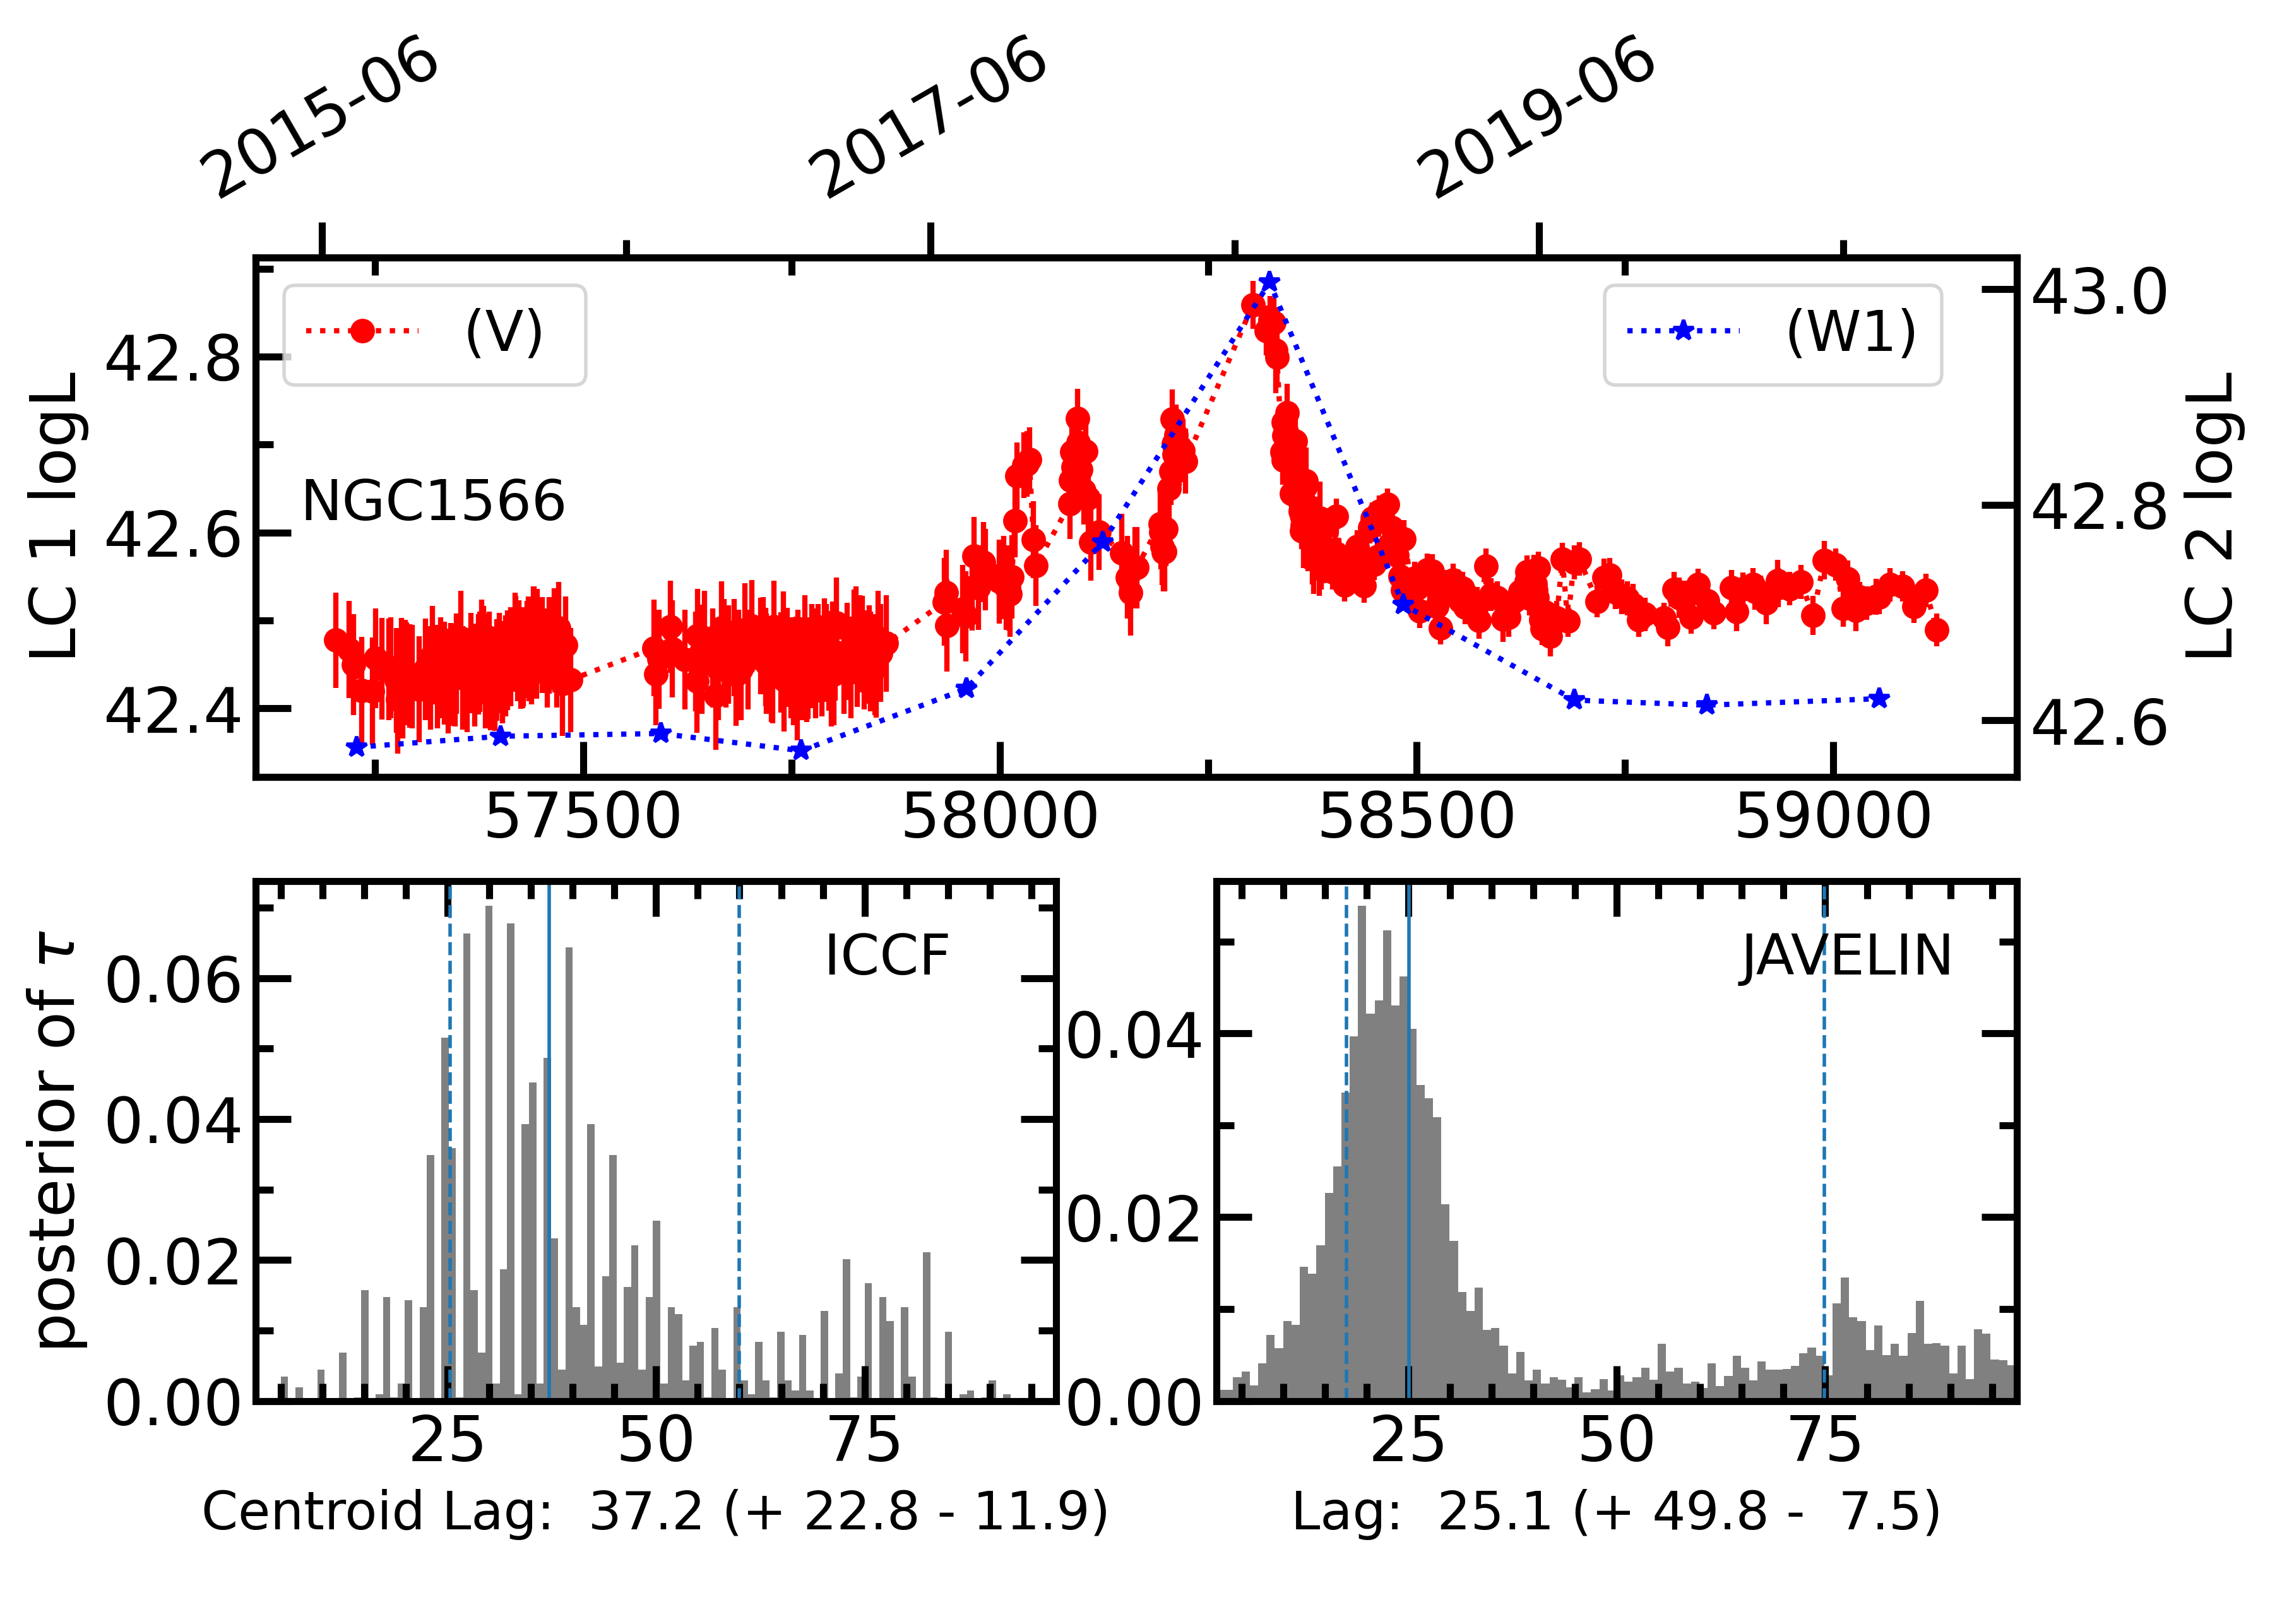
\includegraphics[width=0.5\textwidth]{pic/NGC1566_lag.png}
    \caption{Dust-reverberation time lag analysis for NGC 1566. }
    \label{fig:lag_NGC1566}
\end{figure}

For other sources, we only use the V band data from ASAS-SN and the re-binned $W1$ data in each visit with good observational overlaps to estimate the time lags. For Mrk 6 and PG1535+547, the V band data are binned in 30 days due to their complex short-term variability. The detailed time lag analysis are similar to NGC 1566. The results from ICCF and {\sc javelin} method are roughly consistent (see Figure 7--15), though the ICCF method almost yields a larger errorbar. 


\begin{figure}
\centering
	% To include a figure from a file named example.*
	% Allowable file formats are eps or ps if compiling using latex
	% or pdf, png, jpg if compiling using pdflatex
	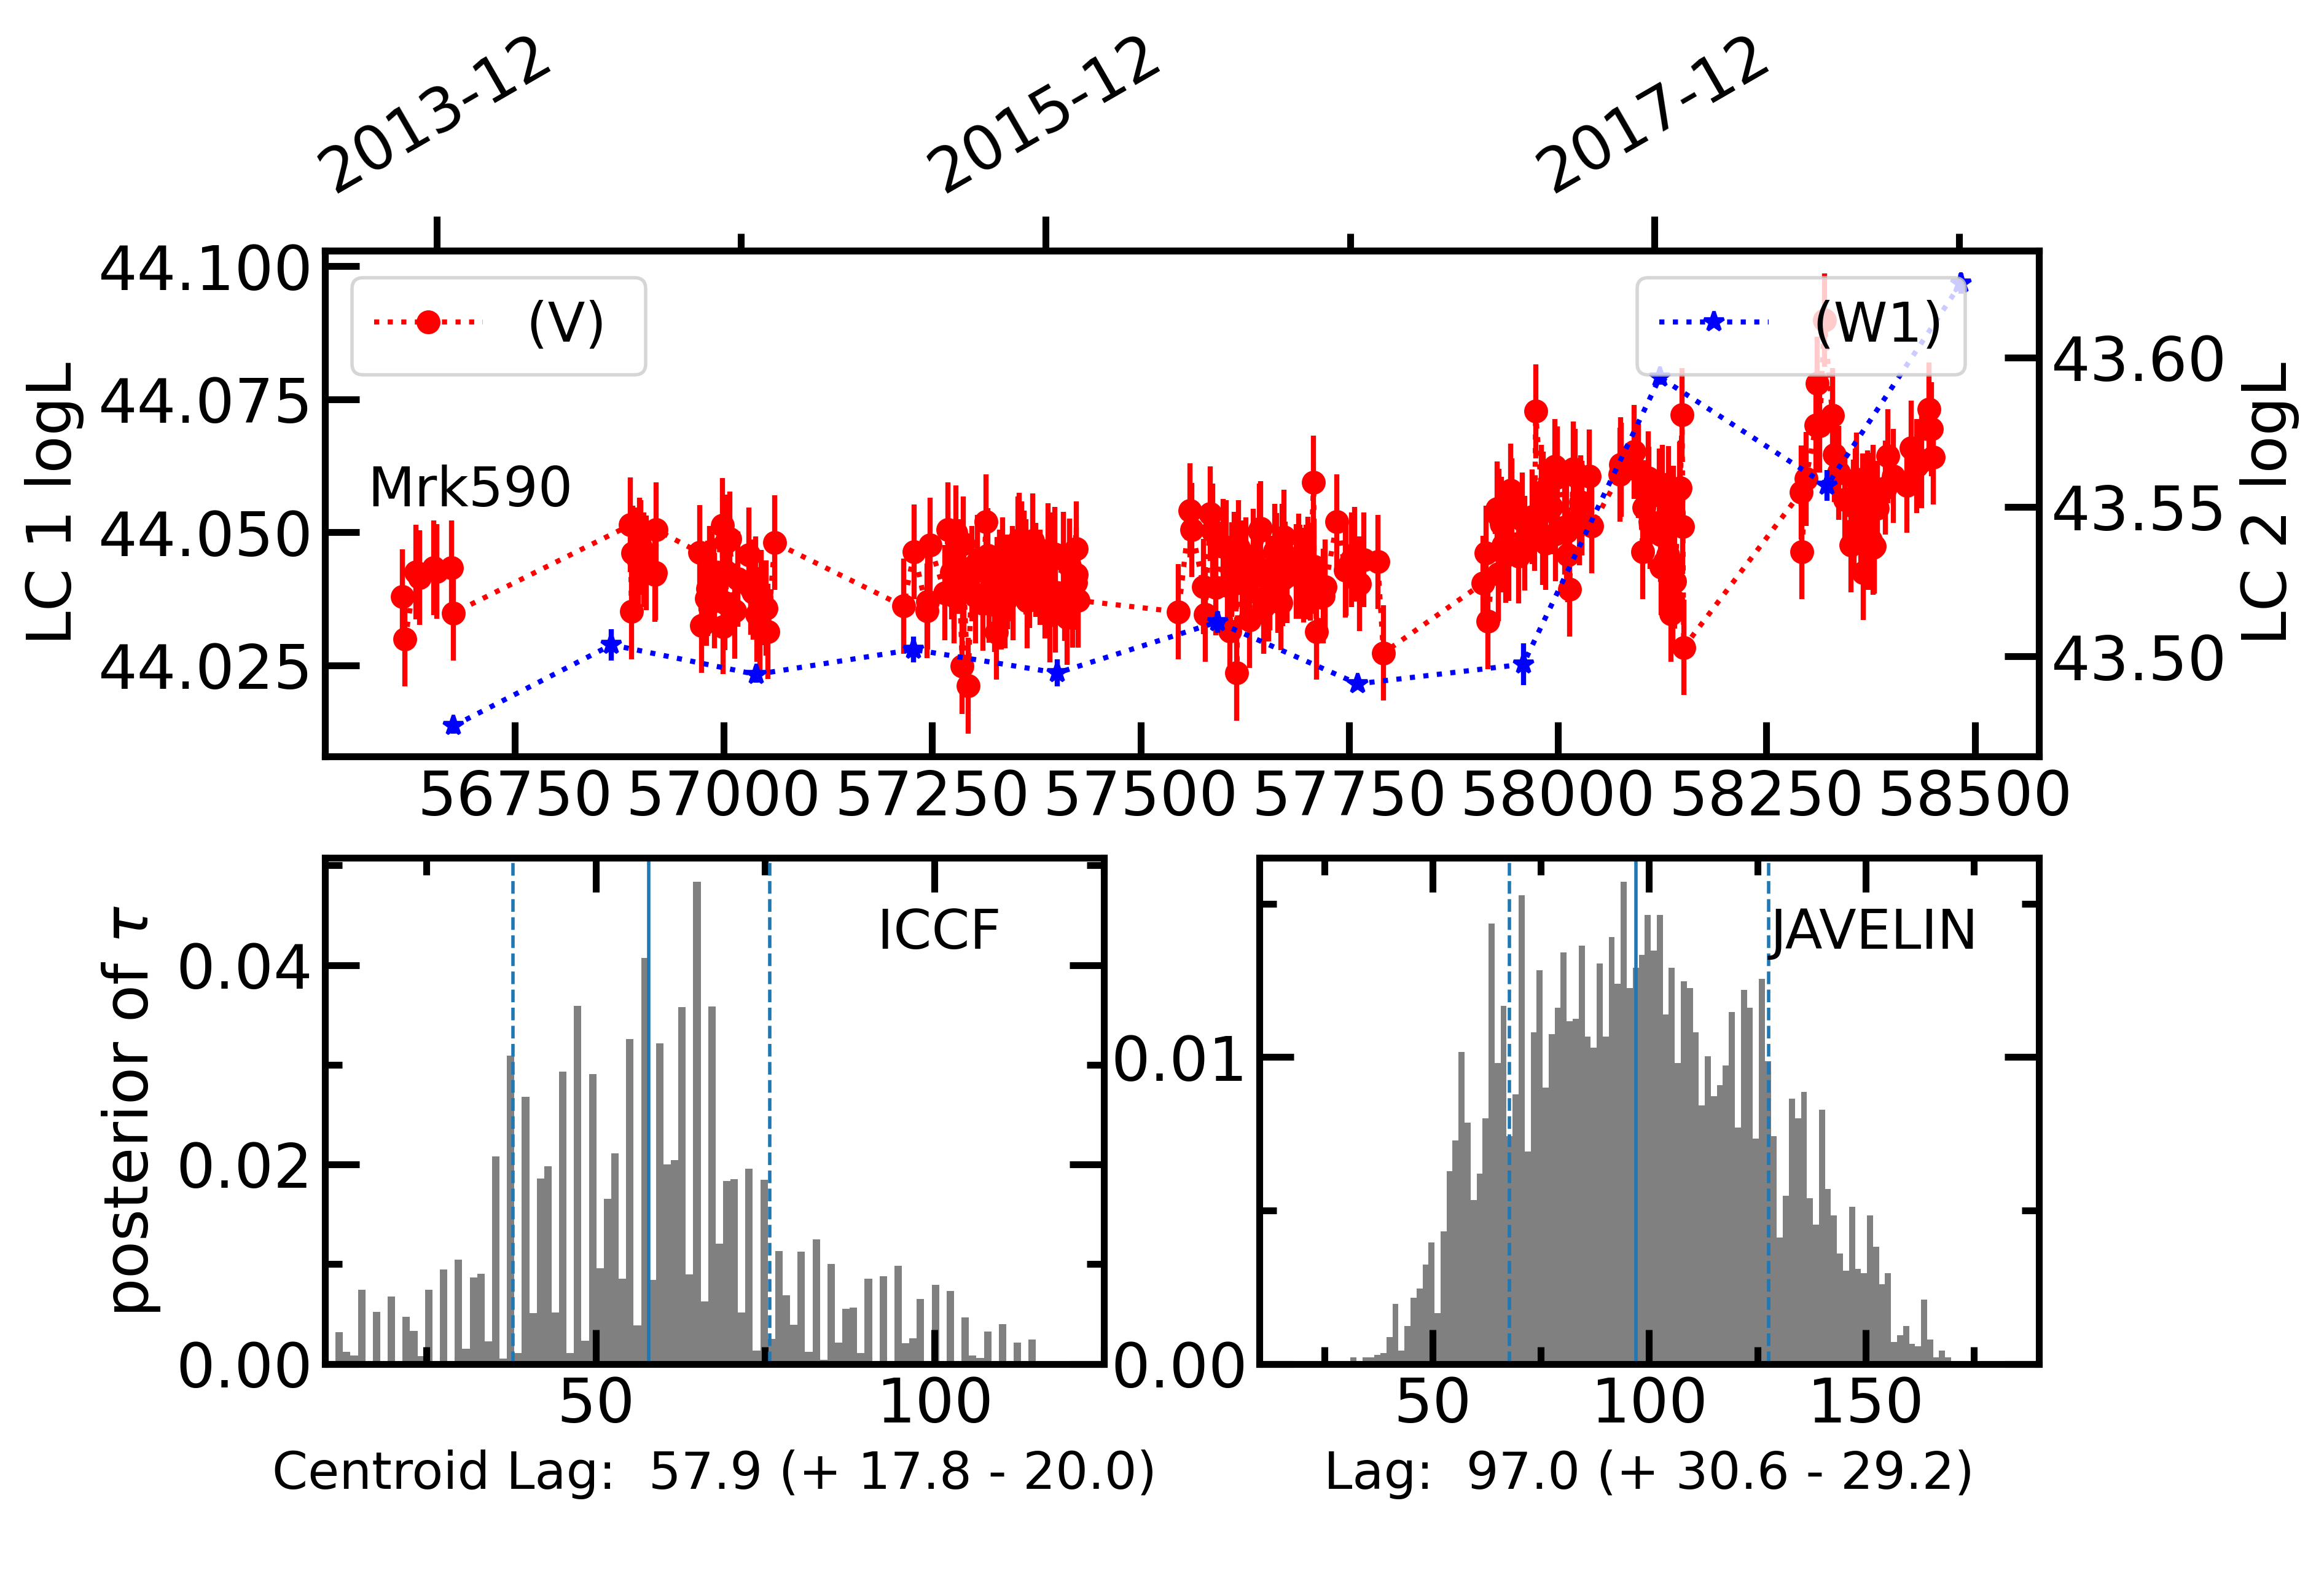
\includegraphics[width=0.5\textwidth]{pic/Mrk590lag.png}
    \caption{Dust-reverberation time lag analysis for Mrk 590. }
    \label{fig:lag_Mrk590}
\end{figure}
\begin{figure}
\centering
	% To include a figure from a file named example.*
	% Allowable file formats are eps or ps if compiling using latex
	% or pdf, png, jpg if compiling using pdflatex
	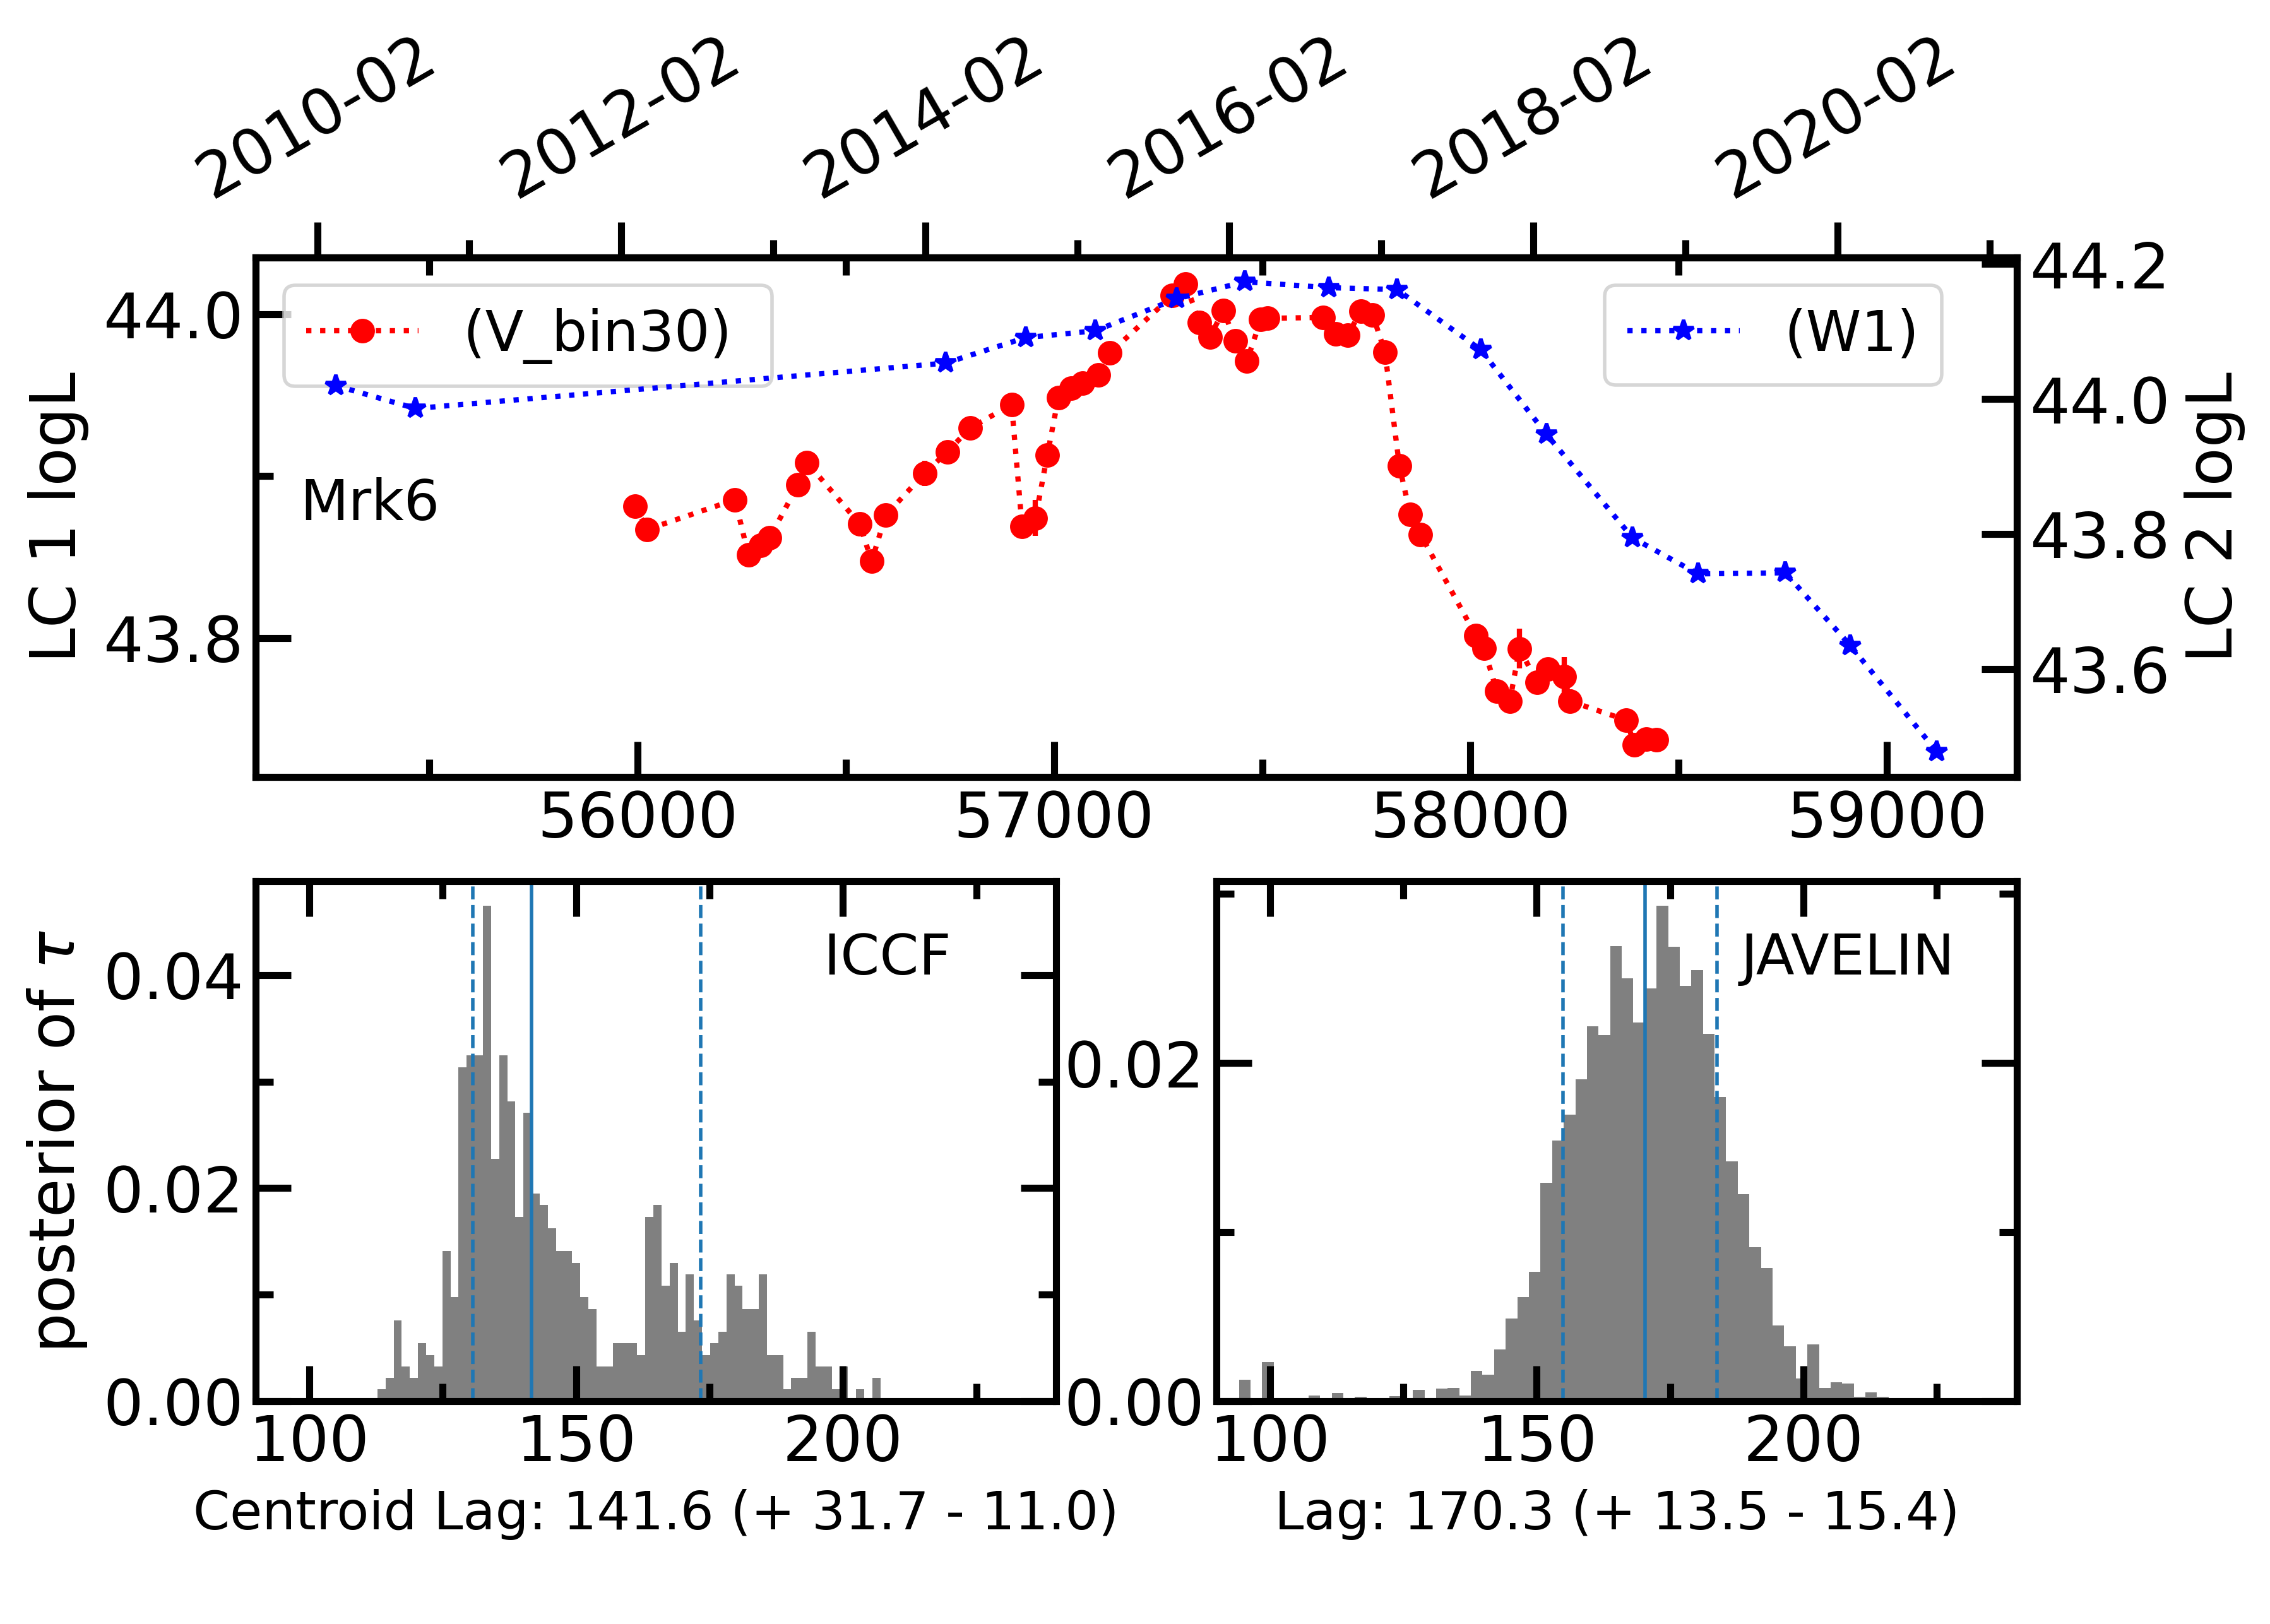
\includegraphics[width=0.5\textwidth]{pic/Mrk6lag1.png}
    \caption{Dust-reverberation time lag analysis for Mrk 6. }
    \label{fig:lag_Mrk6}
\end{figure}
\begin{figure}
\centering
	% To include a figure from a file named example.*
	% Allowable file formats are eps or ps if compiling using latex
	% or pdf, png, jpg if compiling using pdflatex
	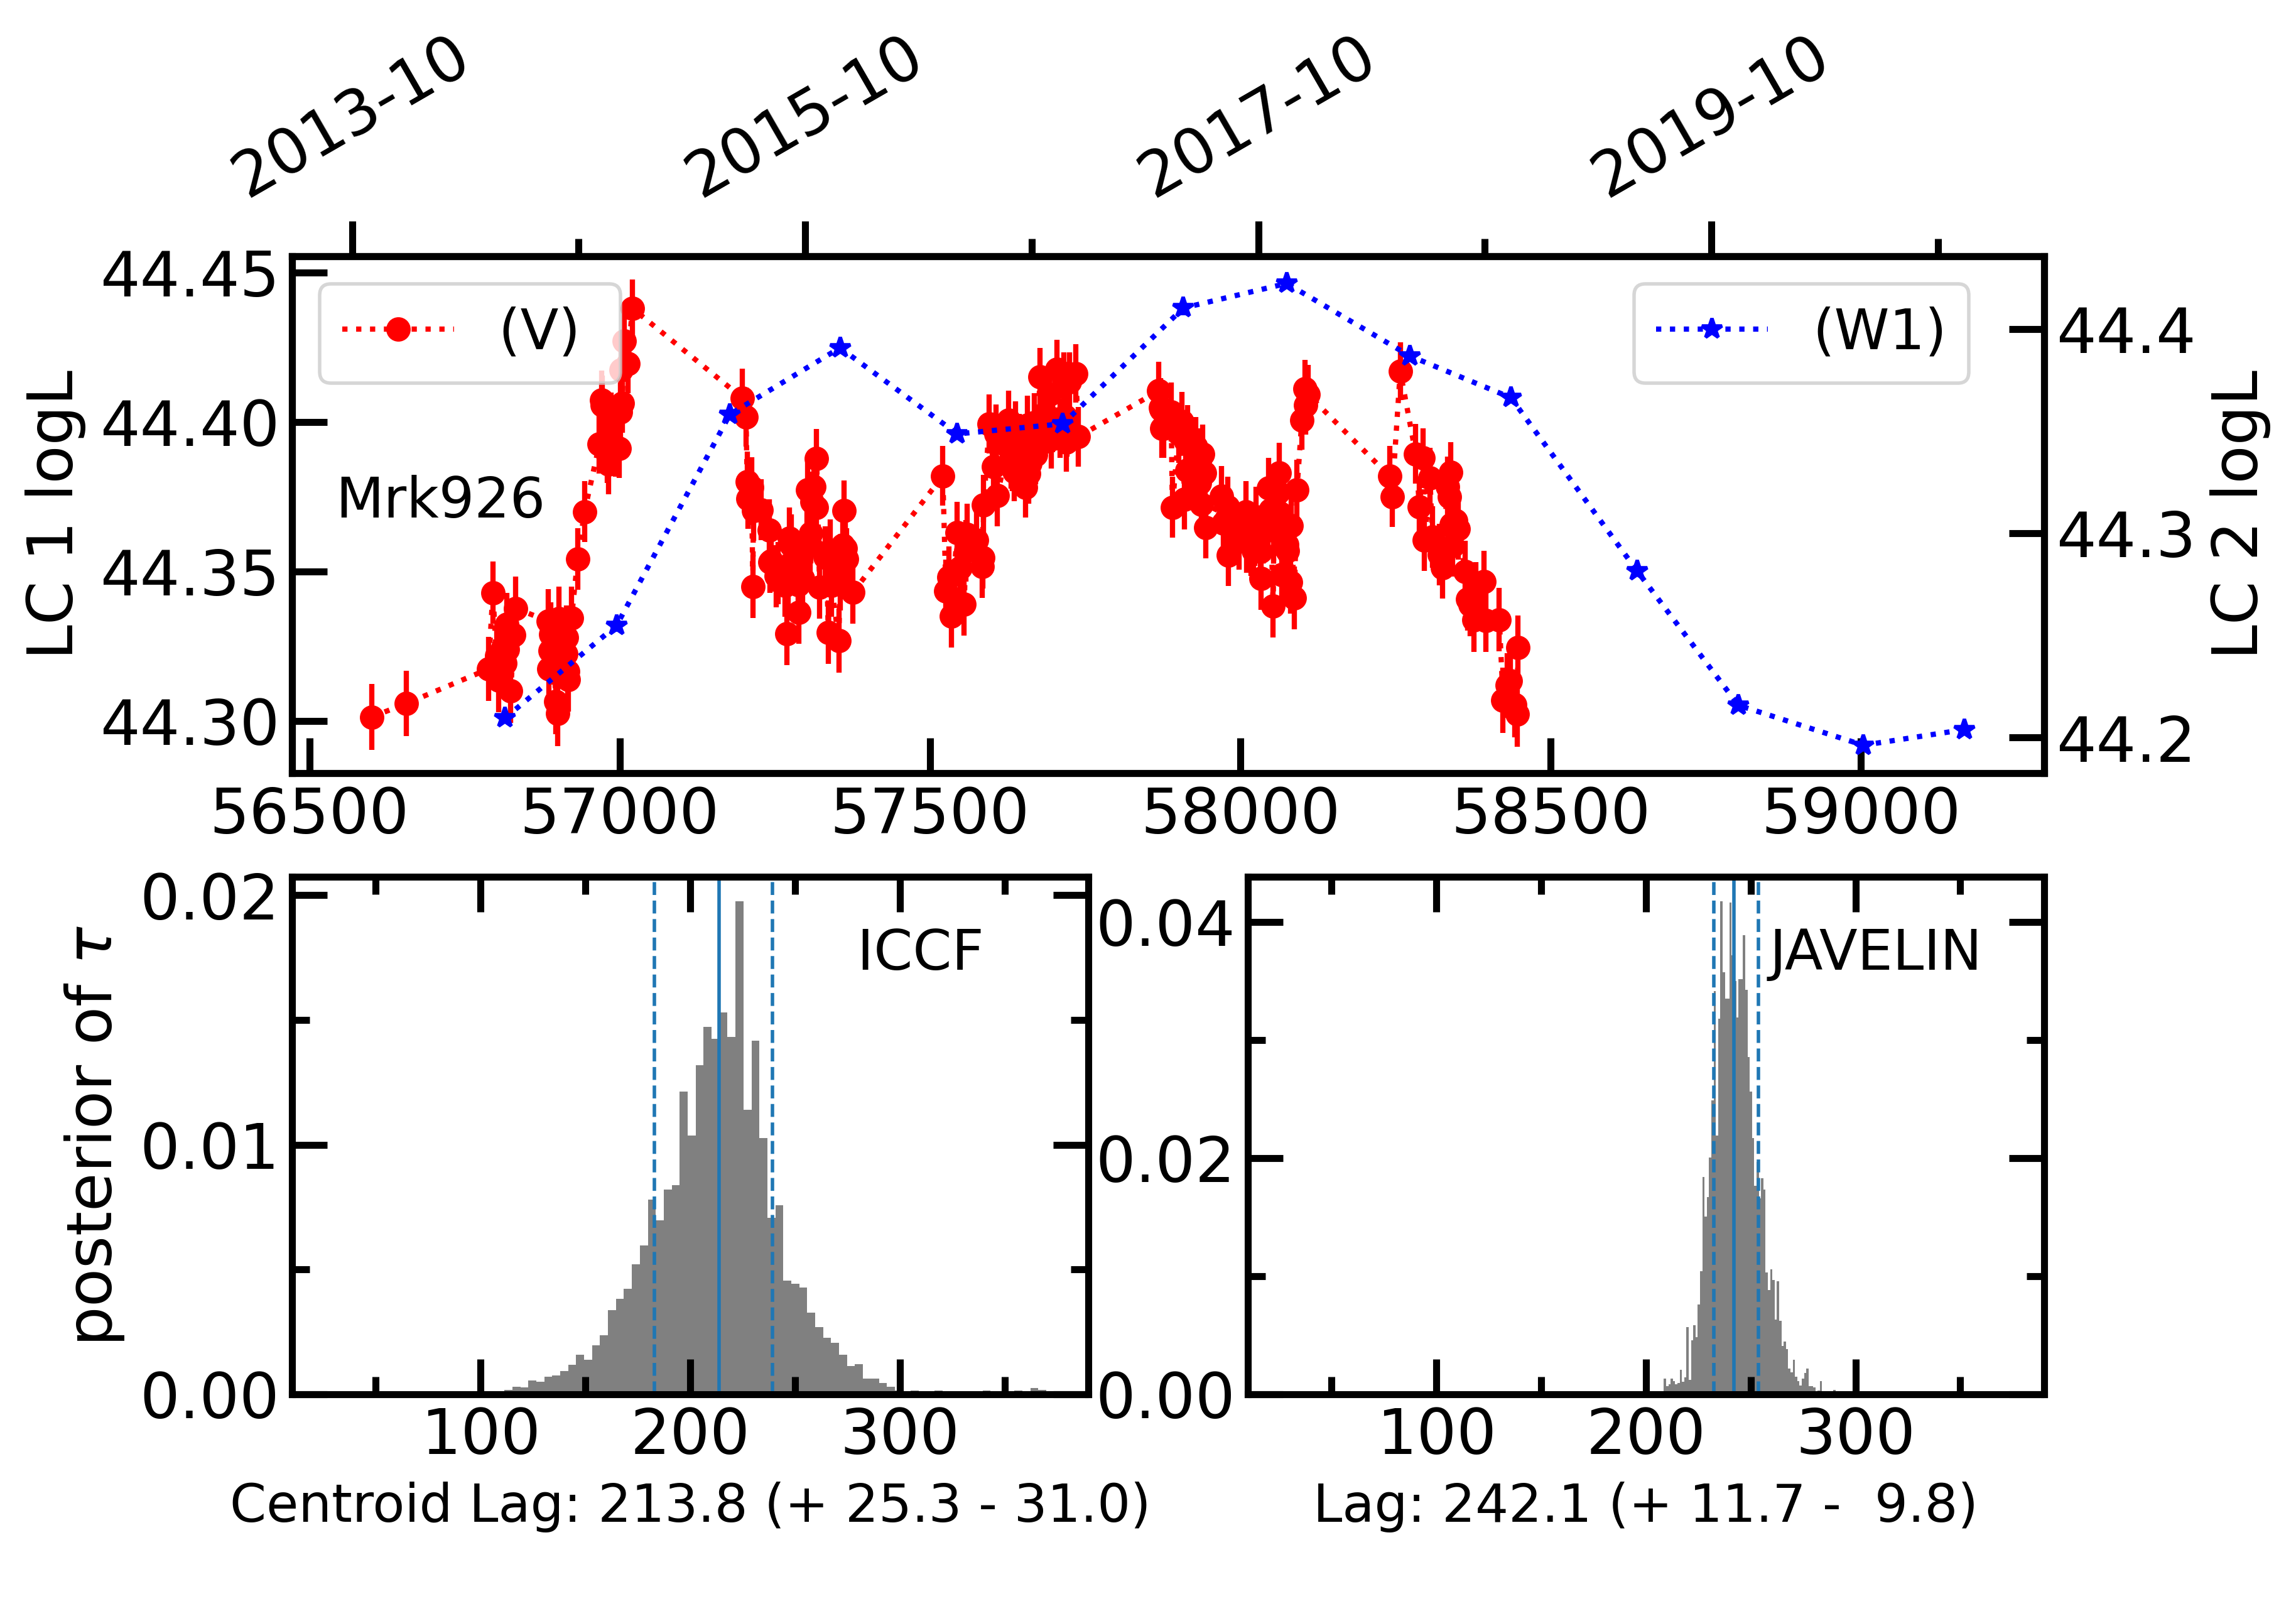
\includegraphics[width=0.5\textwidth]{pic/Mrk926lag.png}
    \caption{Dust-reverberation time lag analysis for Mrk 926. }
    \label{fig:lag_Mrk926}
\end{figure}




\begin{figure}
\centering
	% To include a figure from a file named example.*
	% Allowable file formats are eps or ps if compiling using latex
	% or pdf, png, jpg if compiling using pdflatex
	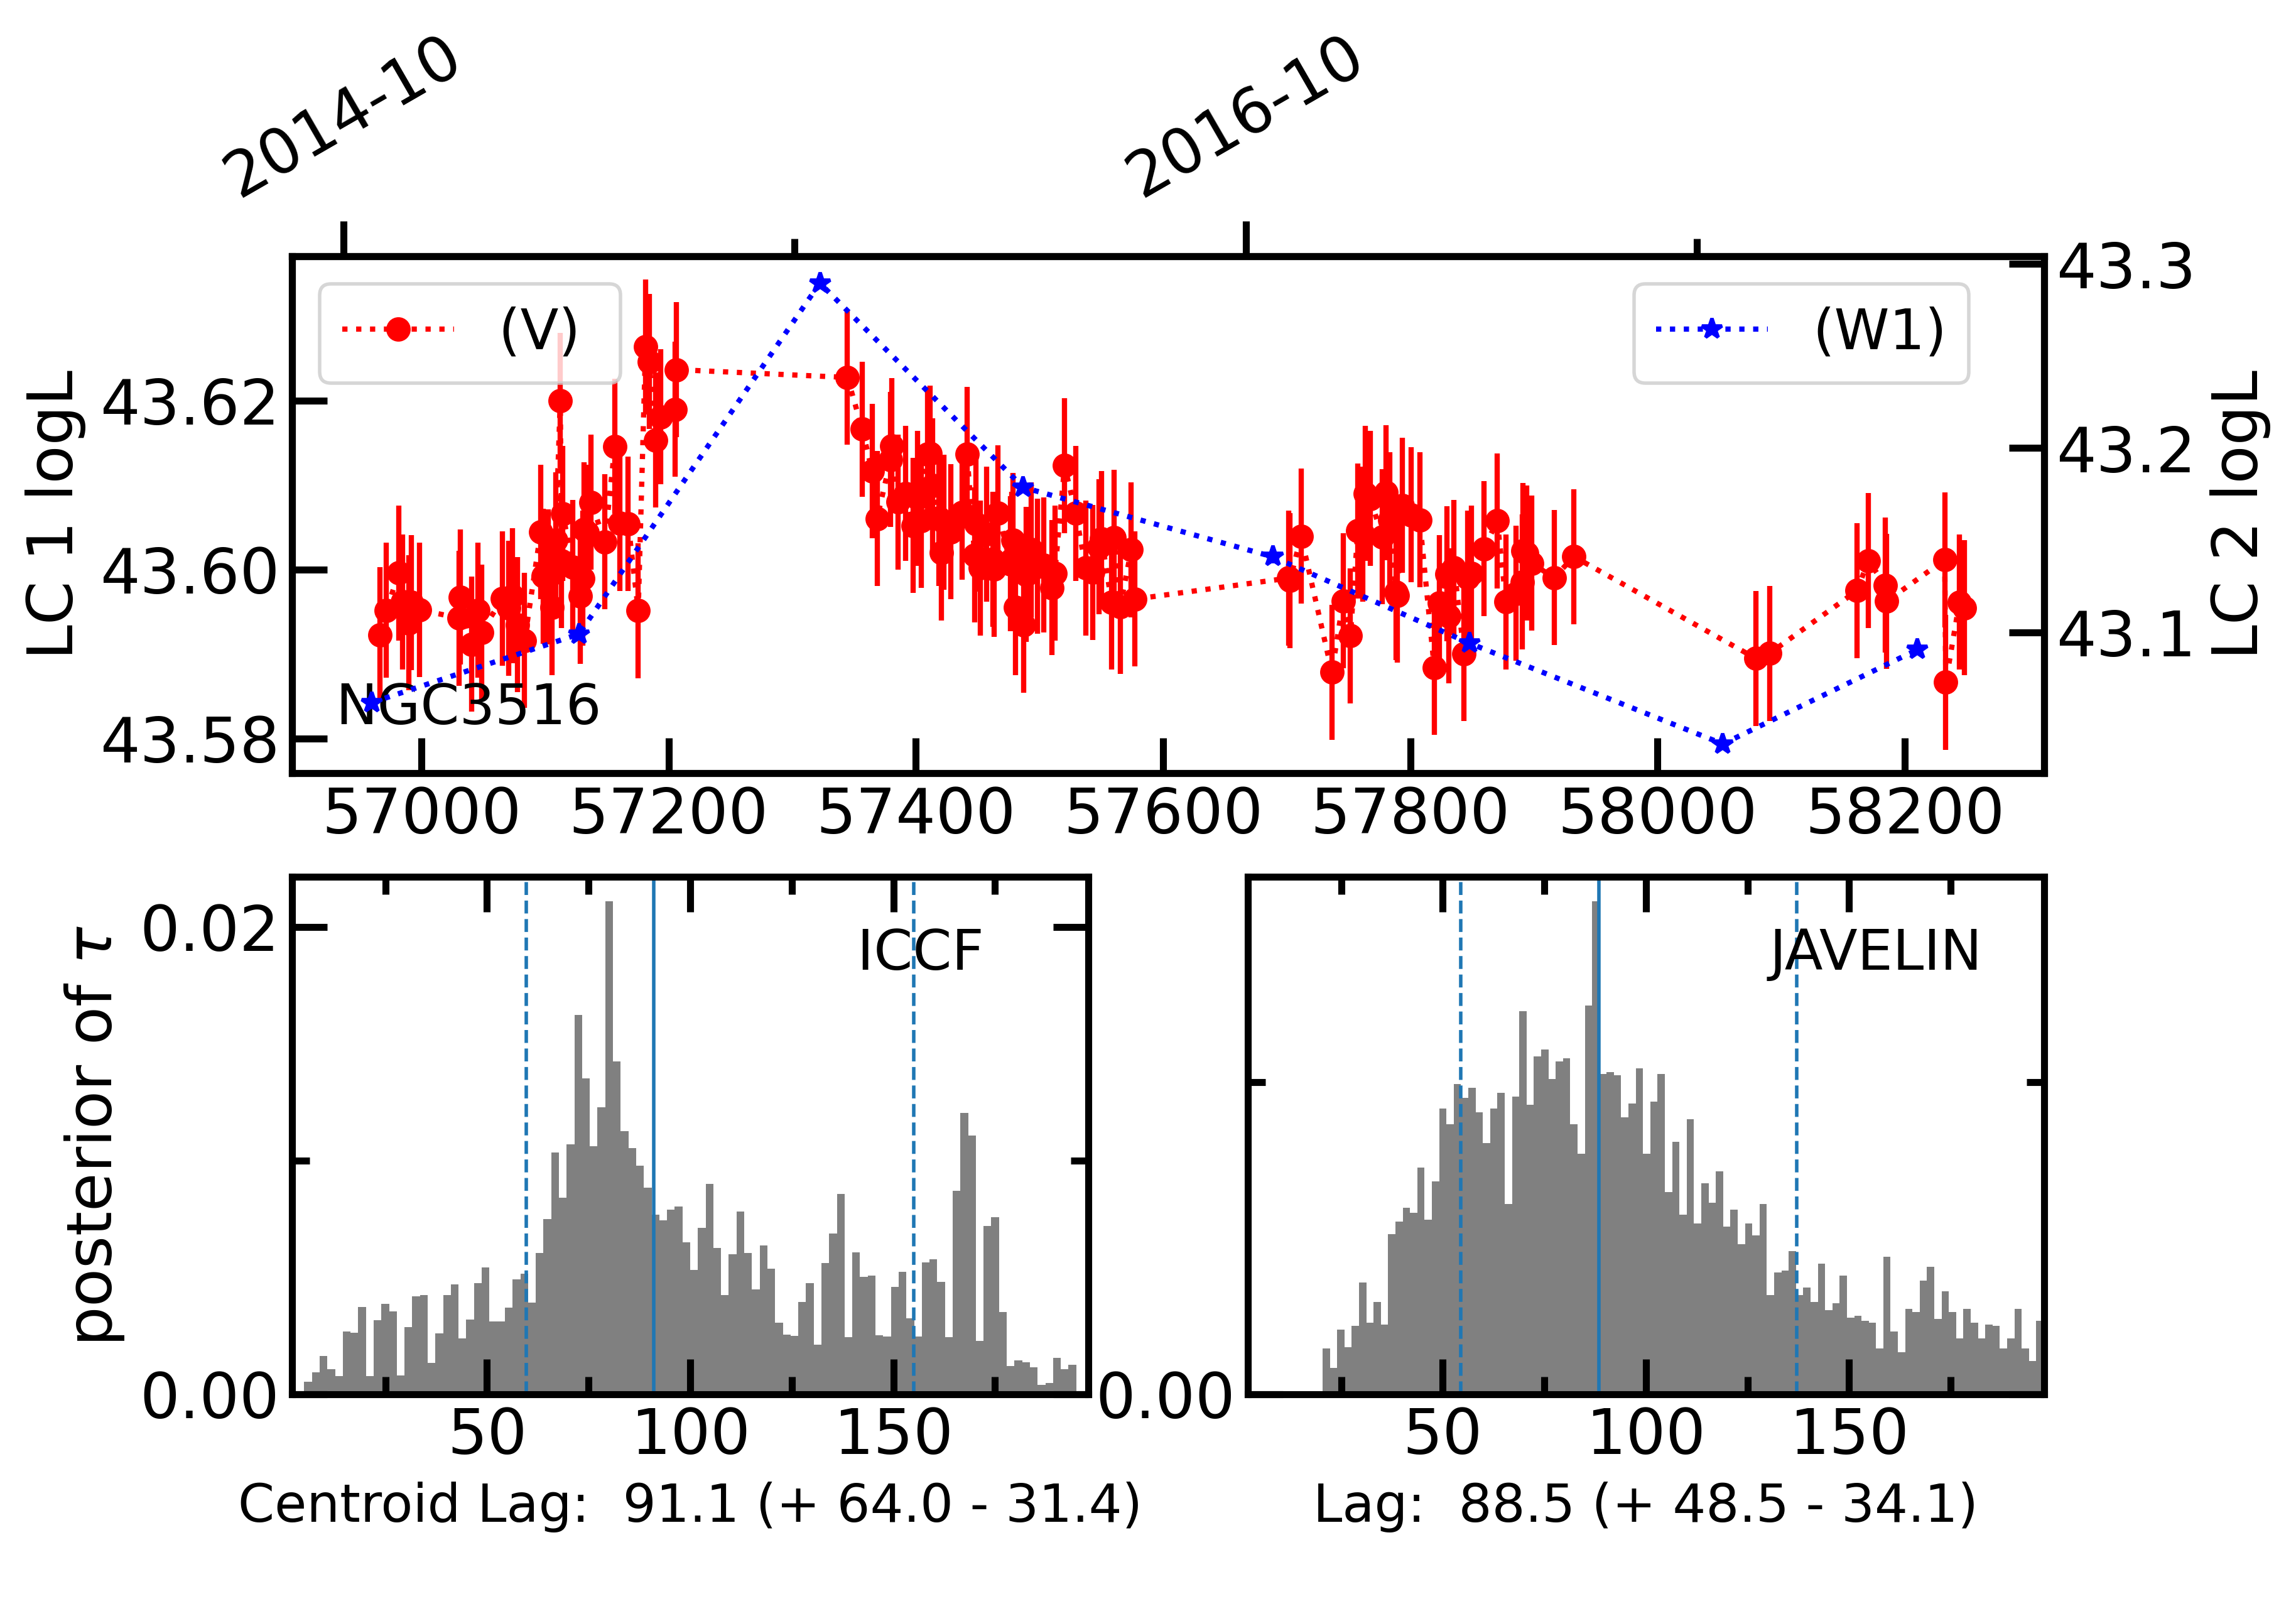
\includegraphics[width=0.5\textwidth]{pic/NGC3516lag.png}
    \caption{Dust-reverberation time lag analysis for NGC 3516. }
    \label{fig:lag_NGC3516}
\end{figure}

\begin{figure}
\centering
	% To include a figure from a file named example.*
	% Allowable file formats are eps or ps if compiling using latex
	% or pdf, png, jpg if compiling using pdflatex
	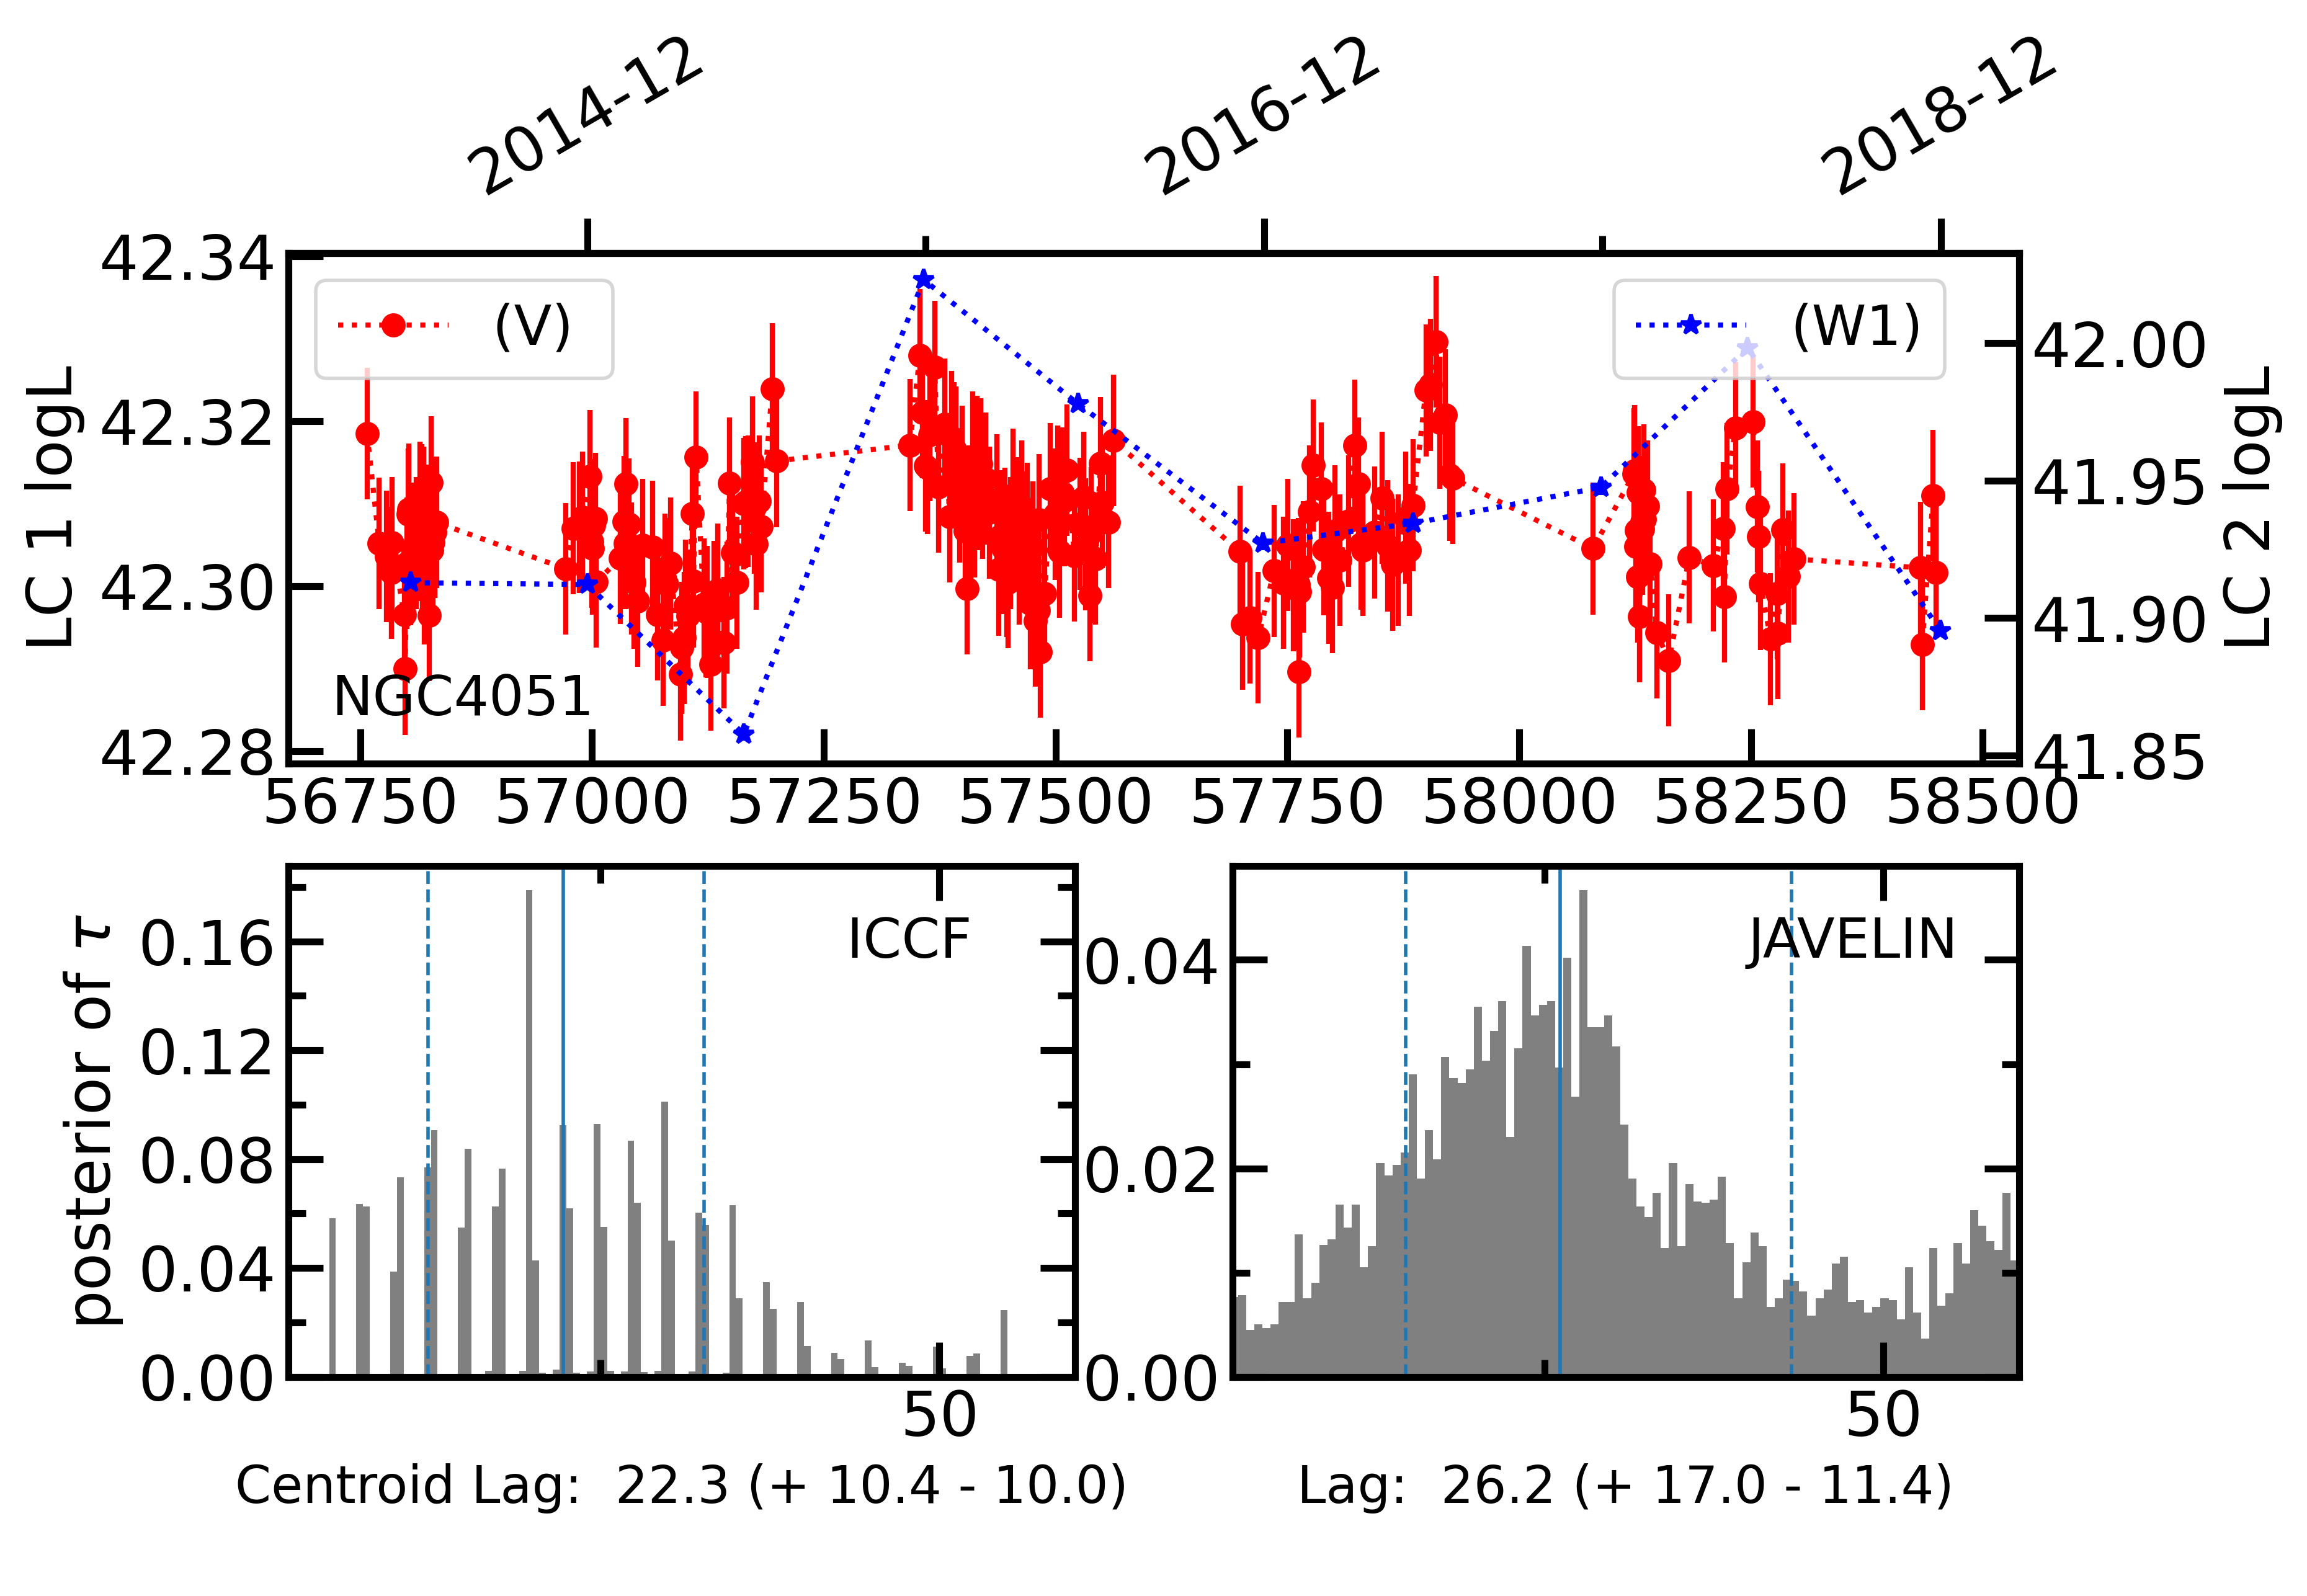
\includegraphics[width=0.5\textwidth]{pic/NGC4051lag.png}
    \caption{Dust-reverberation time lag analysis for NGC 4051. }
    \label{fig:lag_NGC4051}
\end{figure}

\begin{figure}
\centering
	% To include a figure from a file named example.*
	% Allowable file formats are eps or ps if compiling using latex
	% or pdf, png, jpg if compiling using pdflatex
	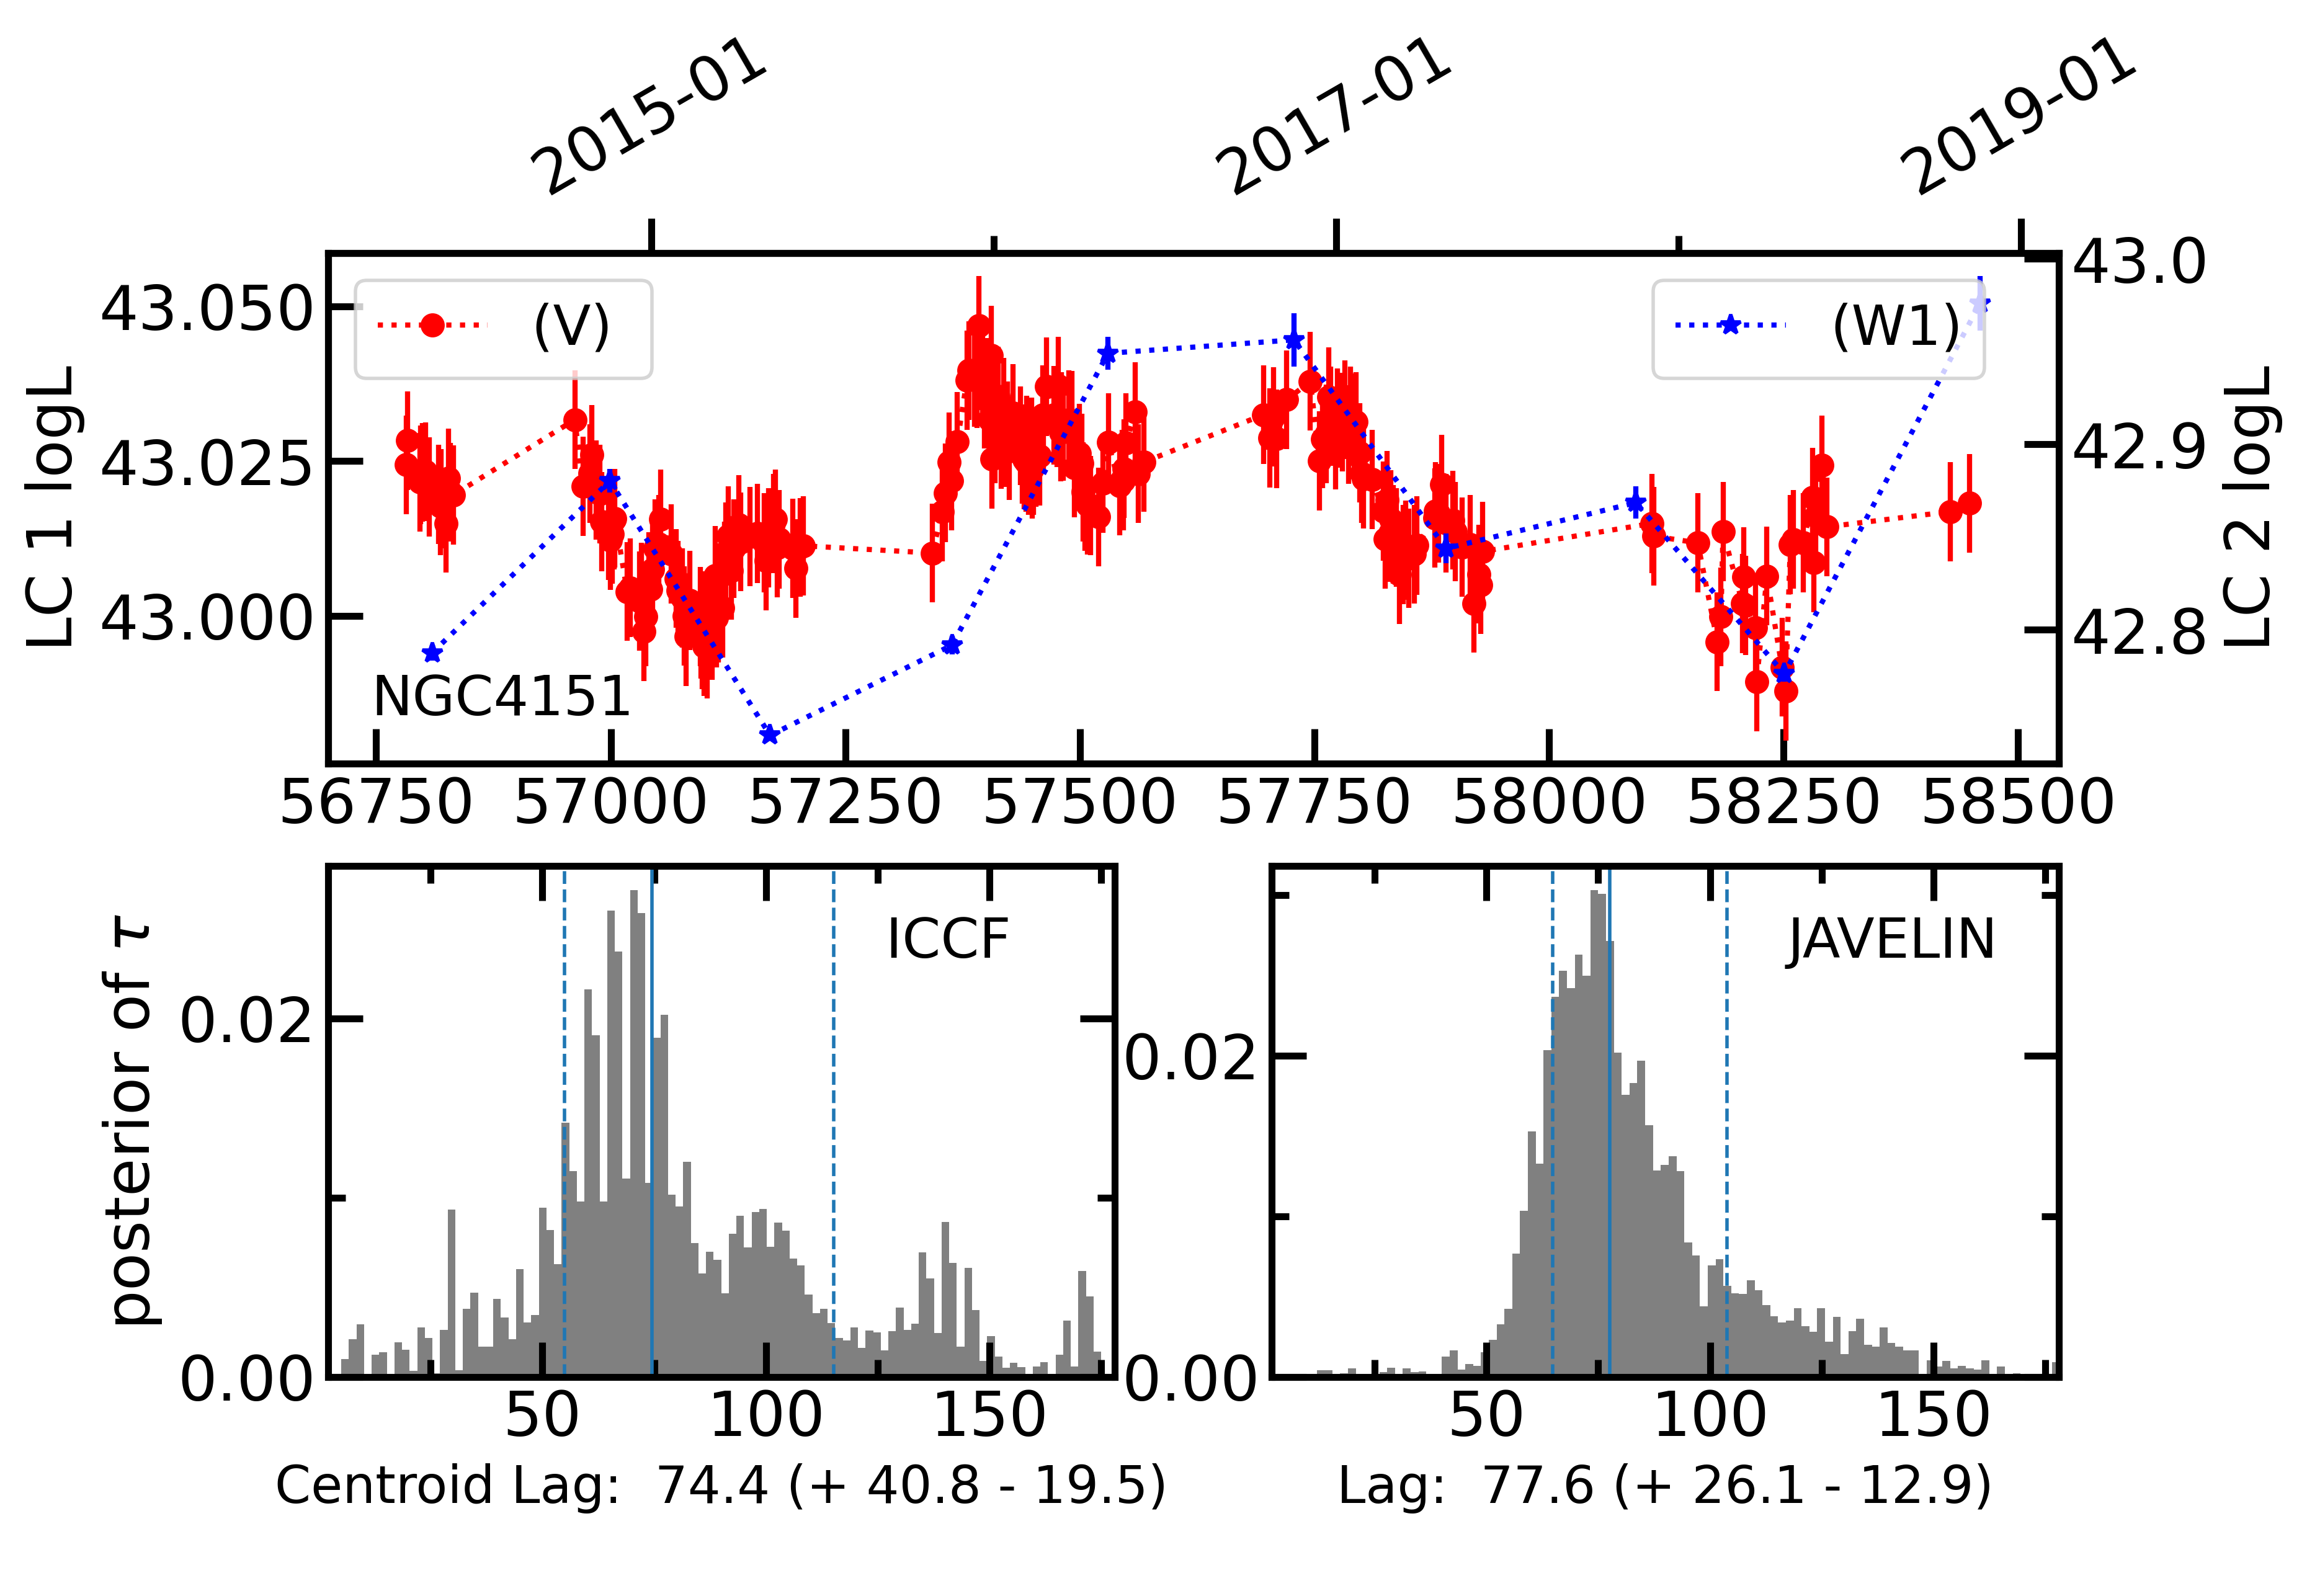
\includegraphics[width=0.5\textwidth]{pic/NGC4151lag.png}
    \caption{Dust-reverberation time lag analysis for NGC 4151. }
    \label{fig:lag_NGC4151}
\end{figure}

\begin{figure}
\centering
	% To include a figure from a file named example.*
	% Allowable file formats are eps or ps if compiling using latex
	% or pdf, png, jpg if compiling using pdflatex
	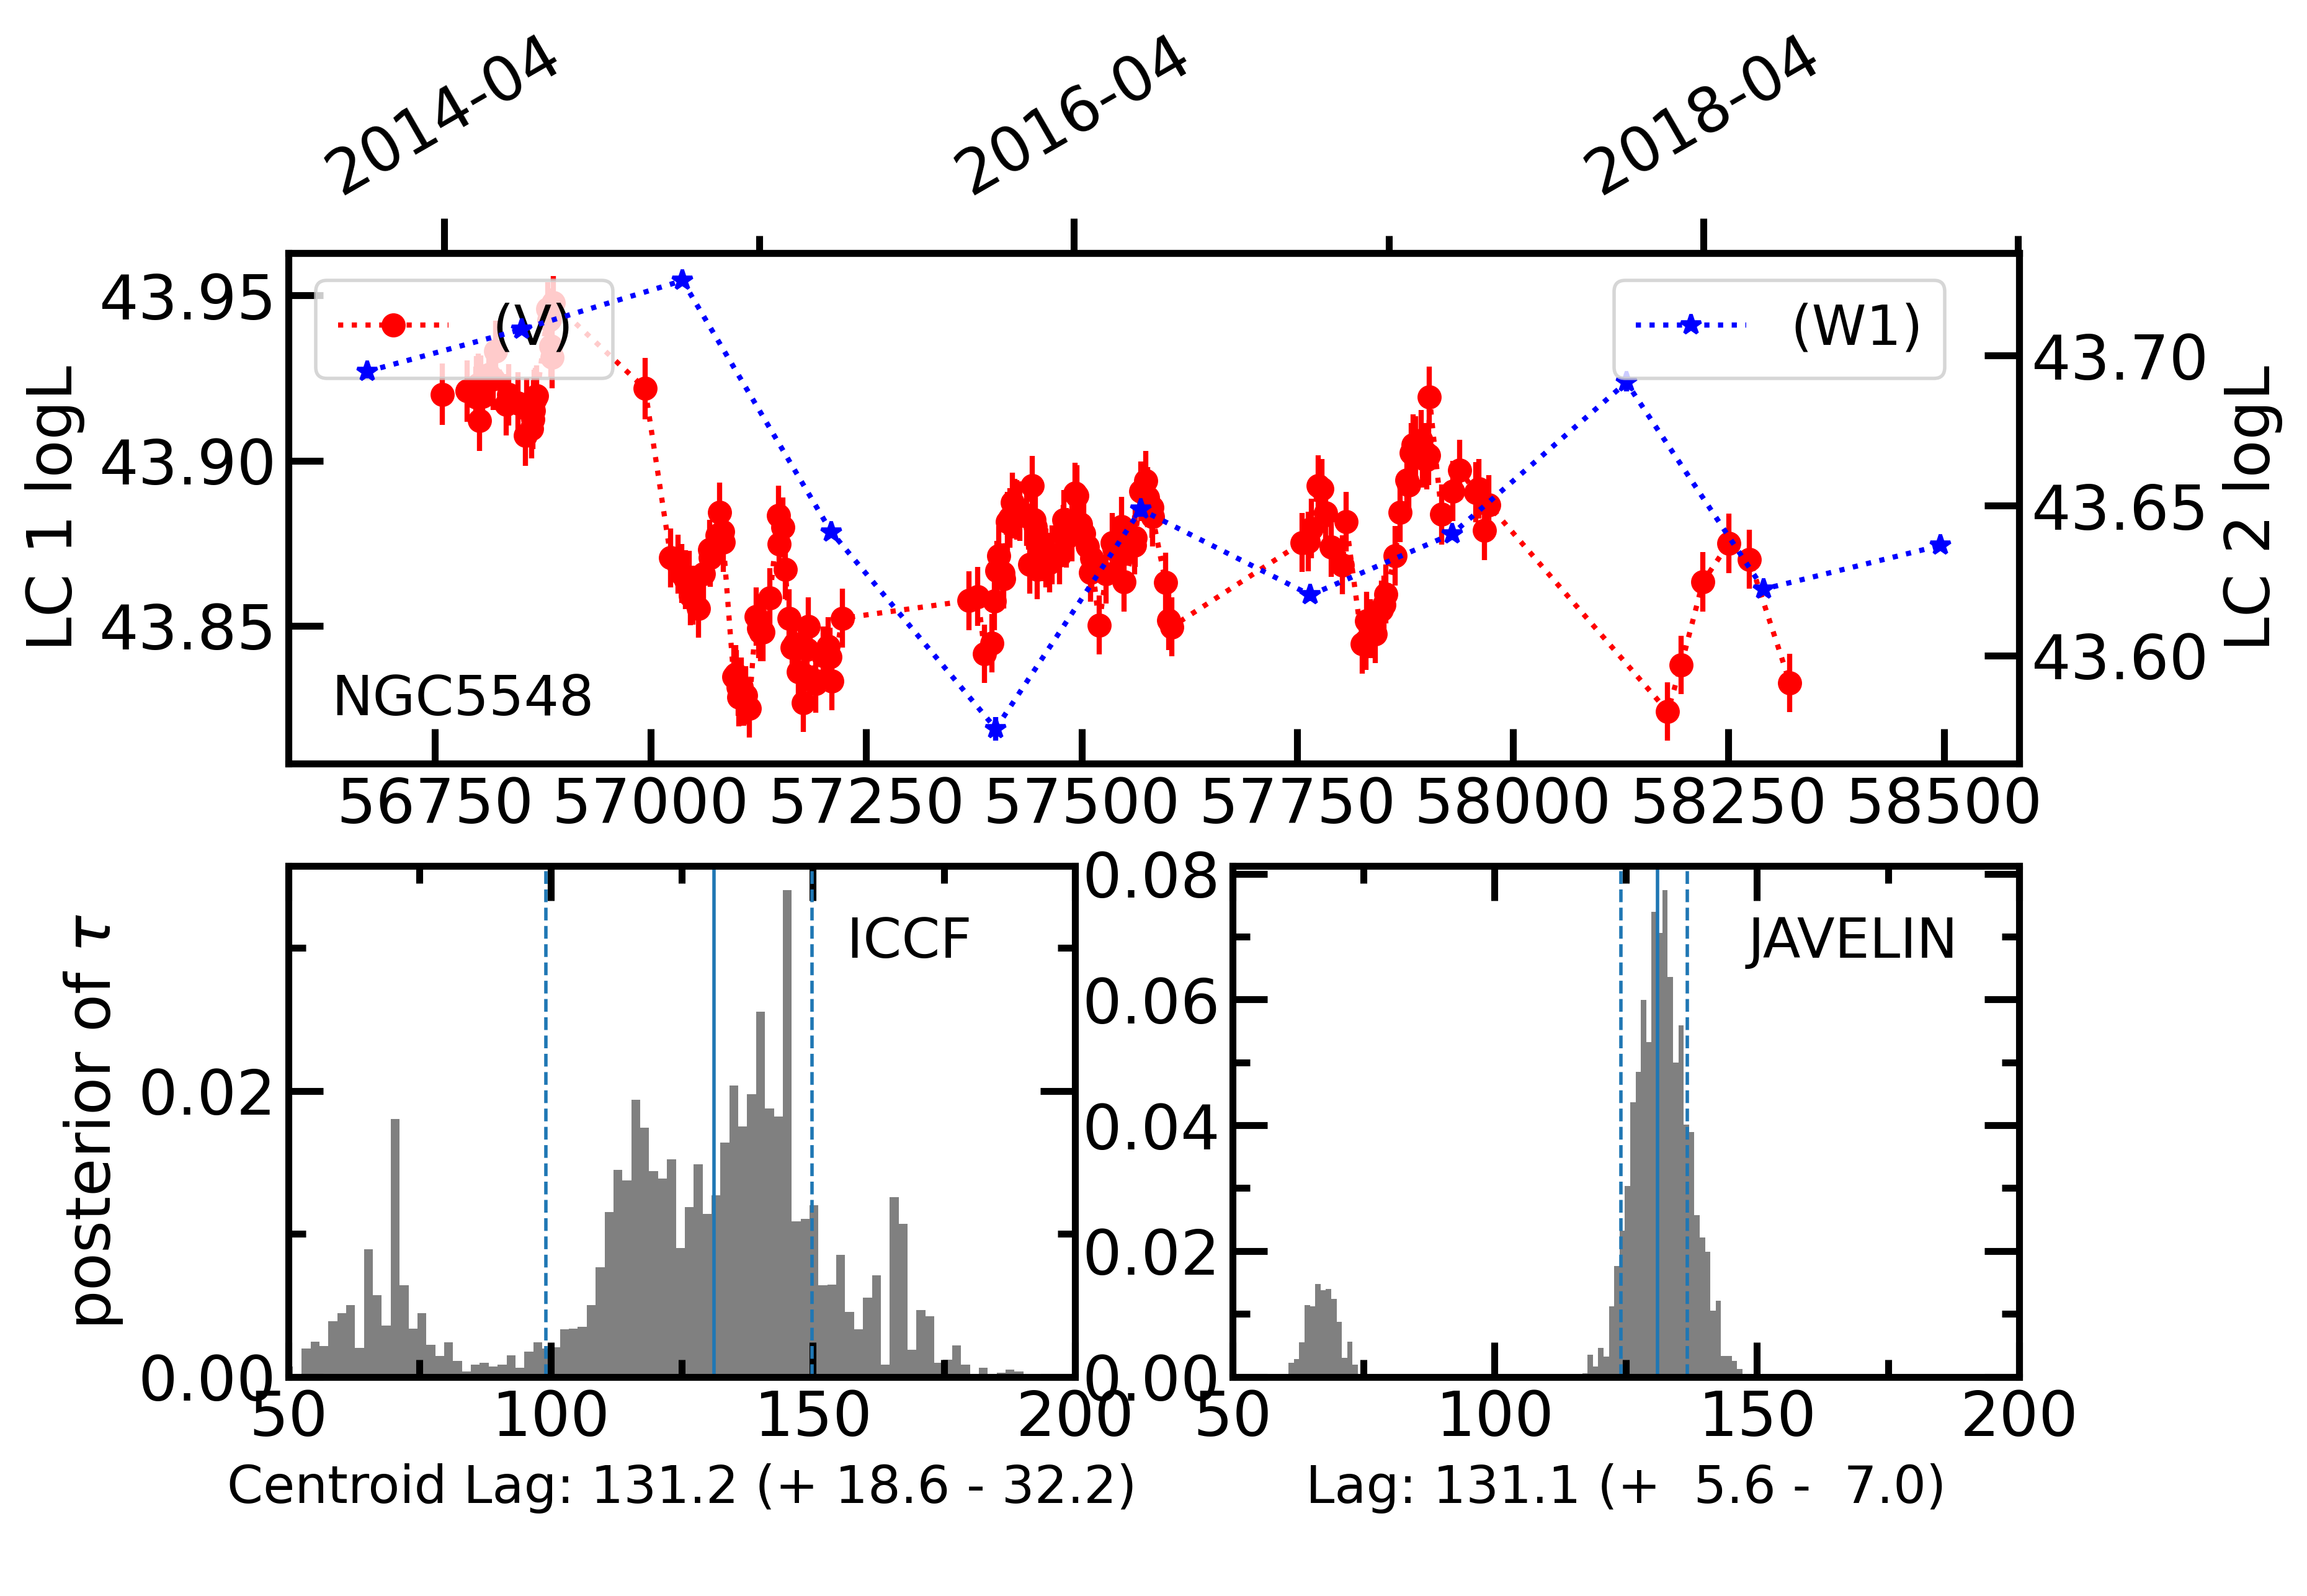
\includegraphics[width=0.5\textwidth]{pic/NGC5548lag.png}
    \caption{Dust-reverberation time lag analysis for NGC 5548. }
    \label{fig:lag_NGC5548}
\end{figure}

\begin{figure}
\centering
	% To include a figure from a file named example.*
	% Allowable file formats are eps or ps if compiling using latex
	% or pdf, png, jpg if compiling using pdflatex
	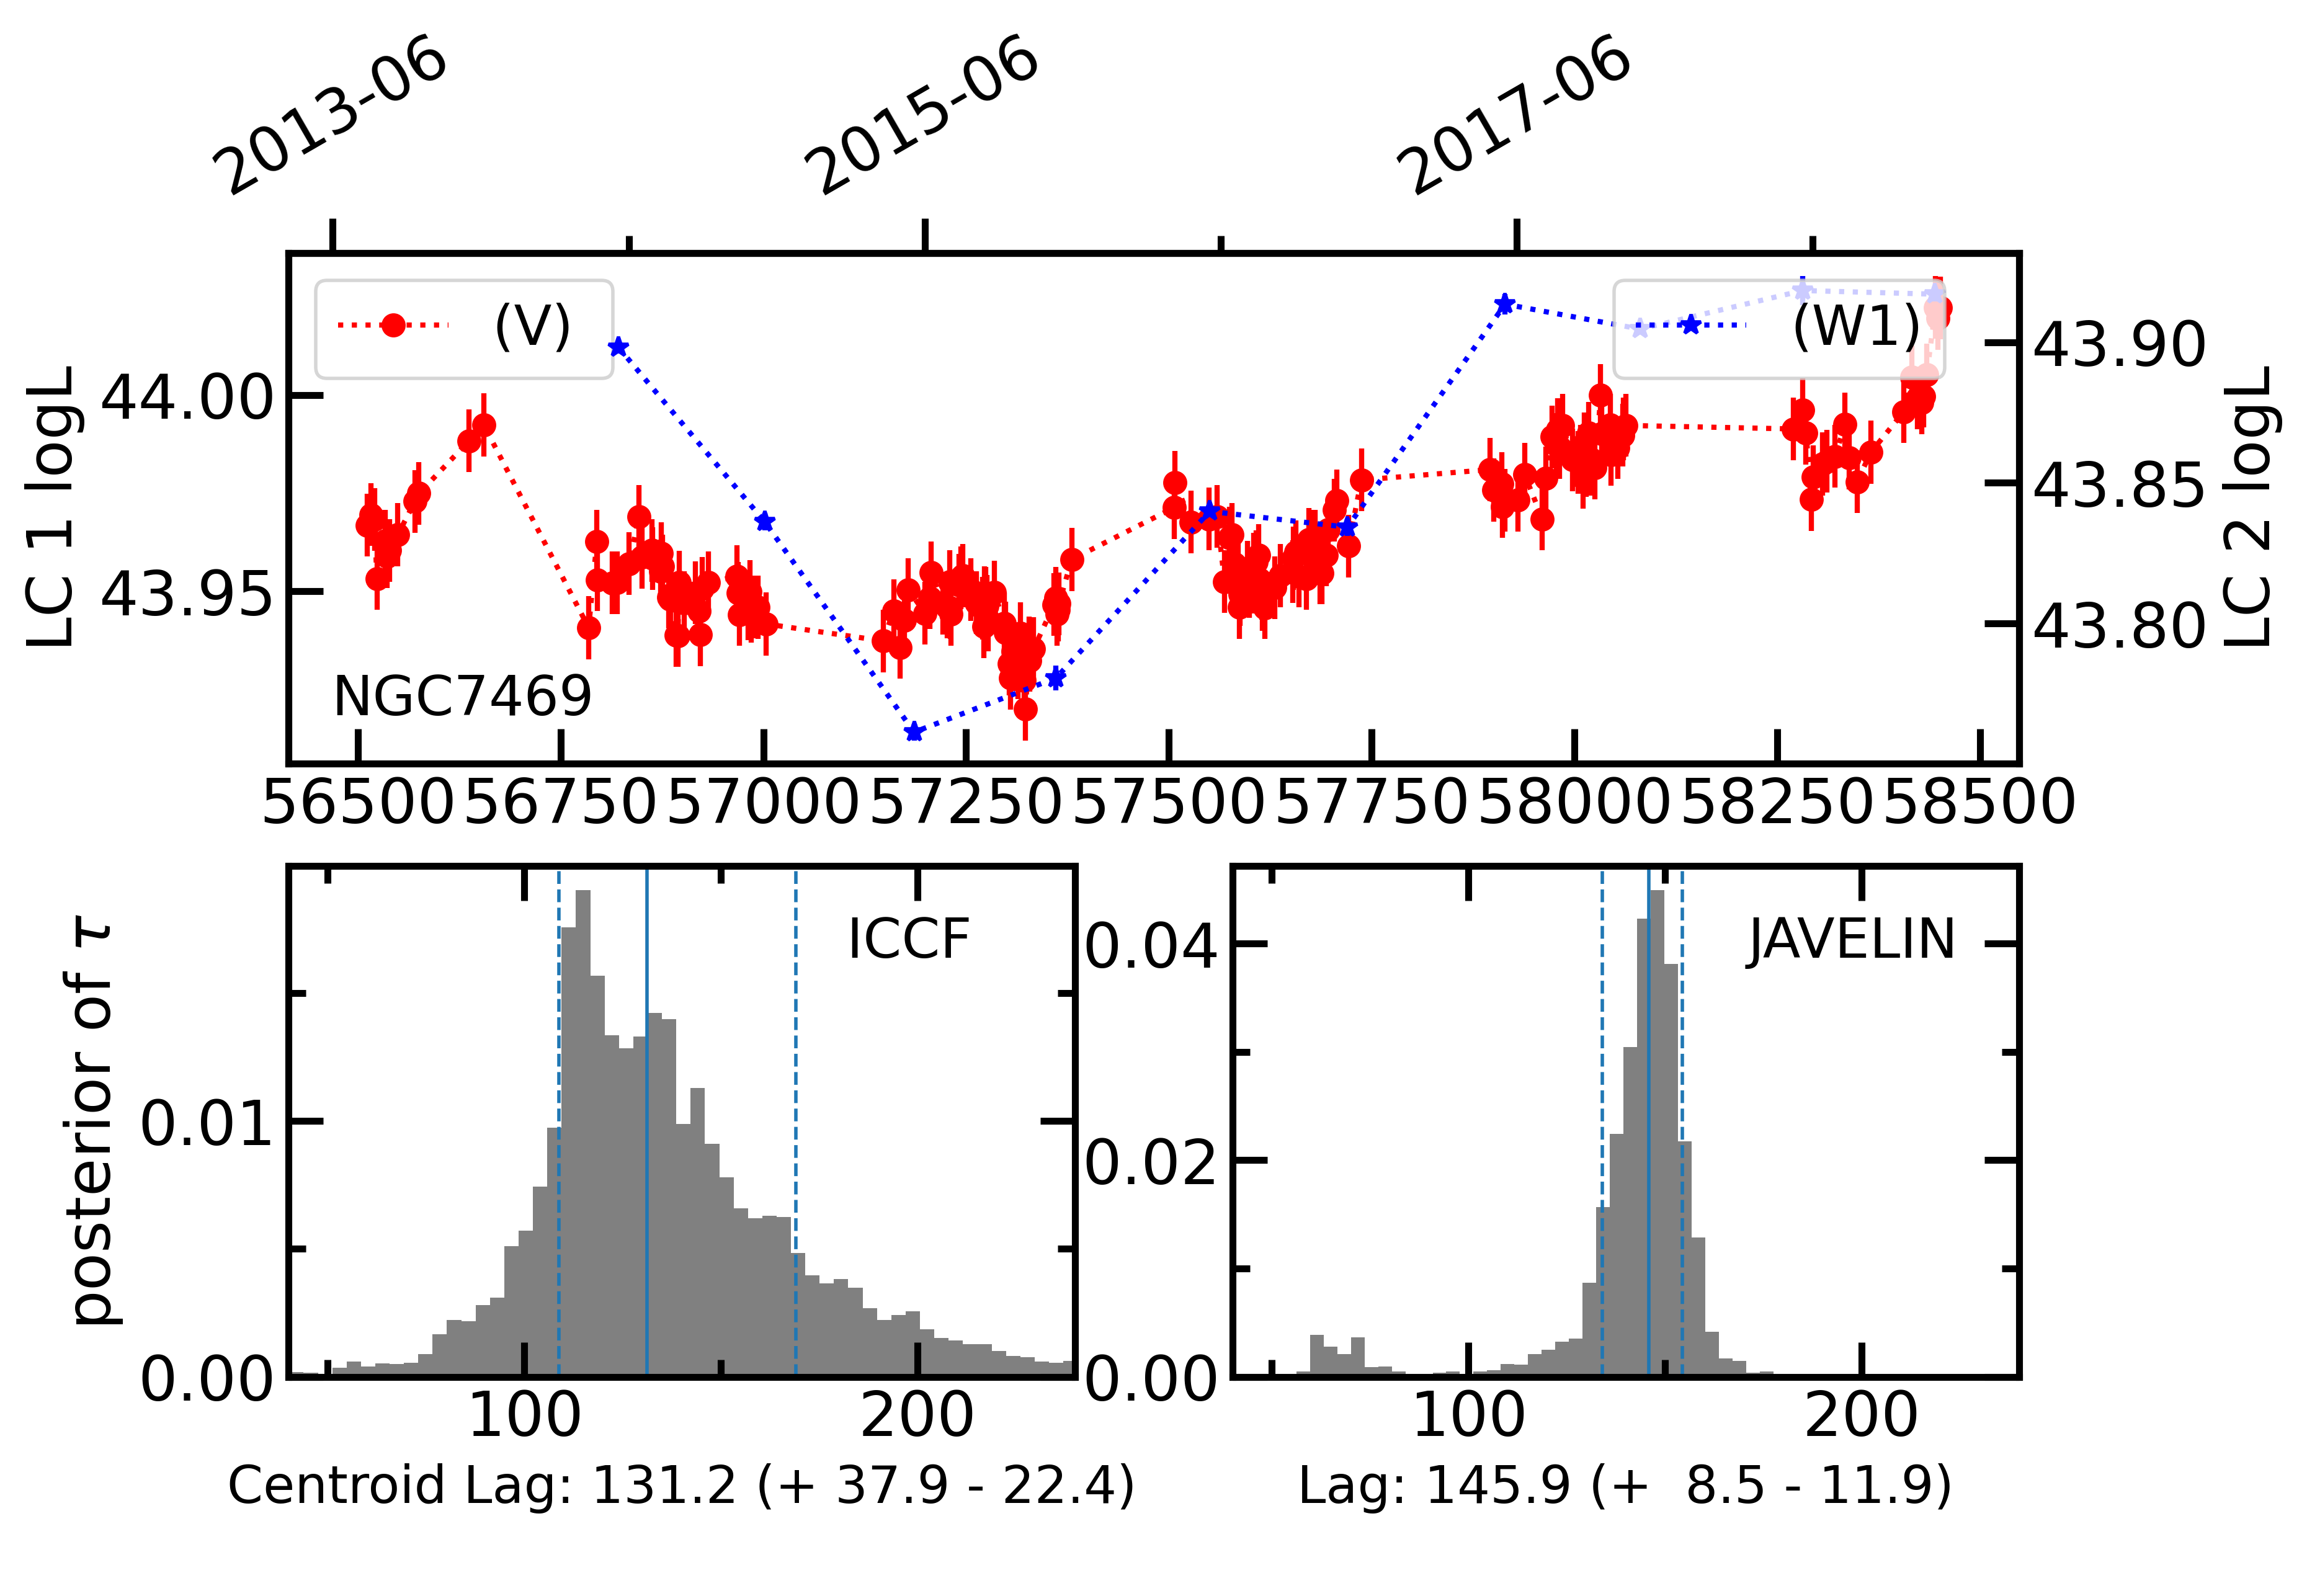
\includegraphics[width=0.5\textwidth]{pic/NGC7469lag.png}
    \caption{Dust-reverberation time lag analysis for NGC 7469. }
    \label{fig:lag_NGC7469}
\end{figure}
\begin{figure}
\centering
	% To include a figure from a file named example.*
	% Allowable file formats are eps or ps if compiling using latex
	% or pdf, png, jpg if compiling using pdflatex
	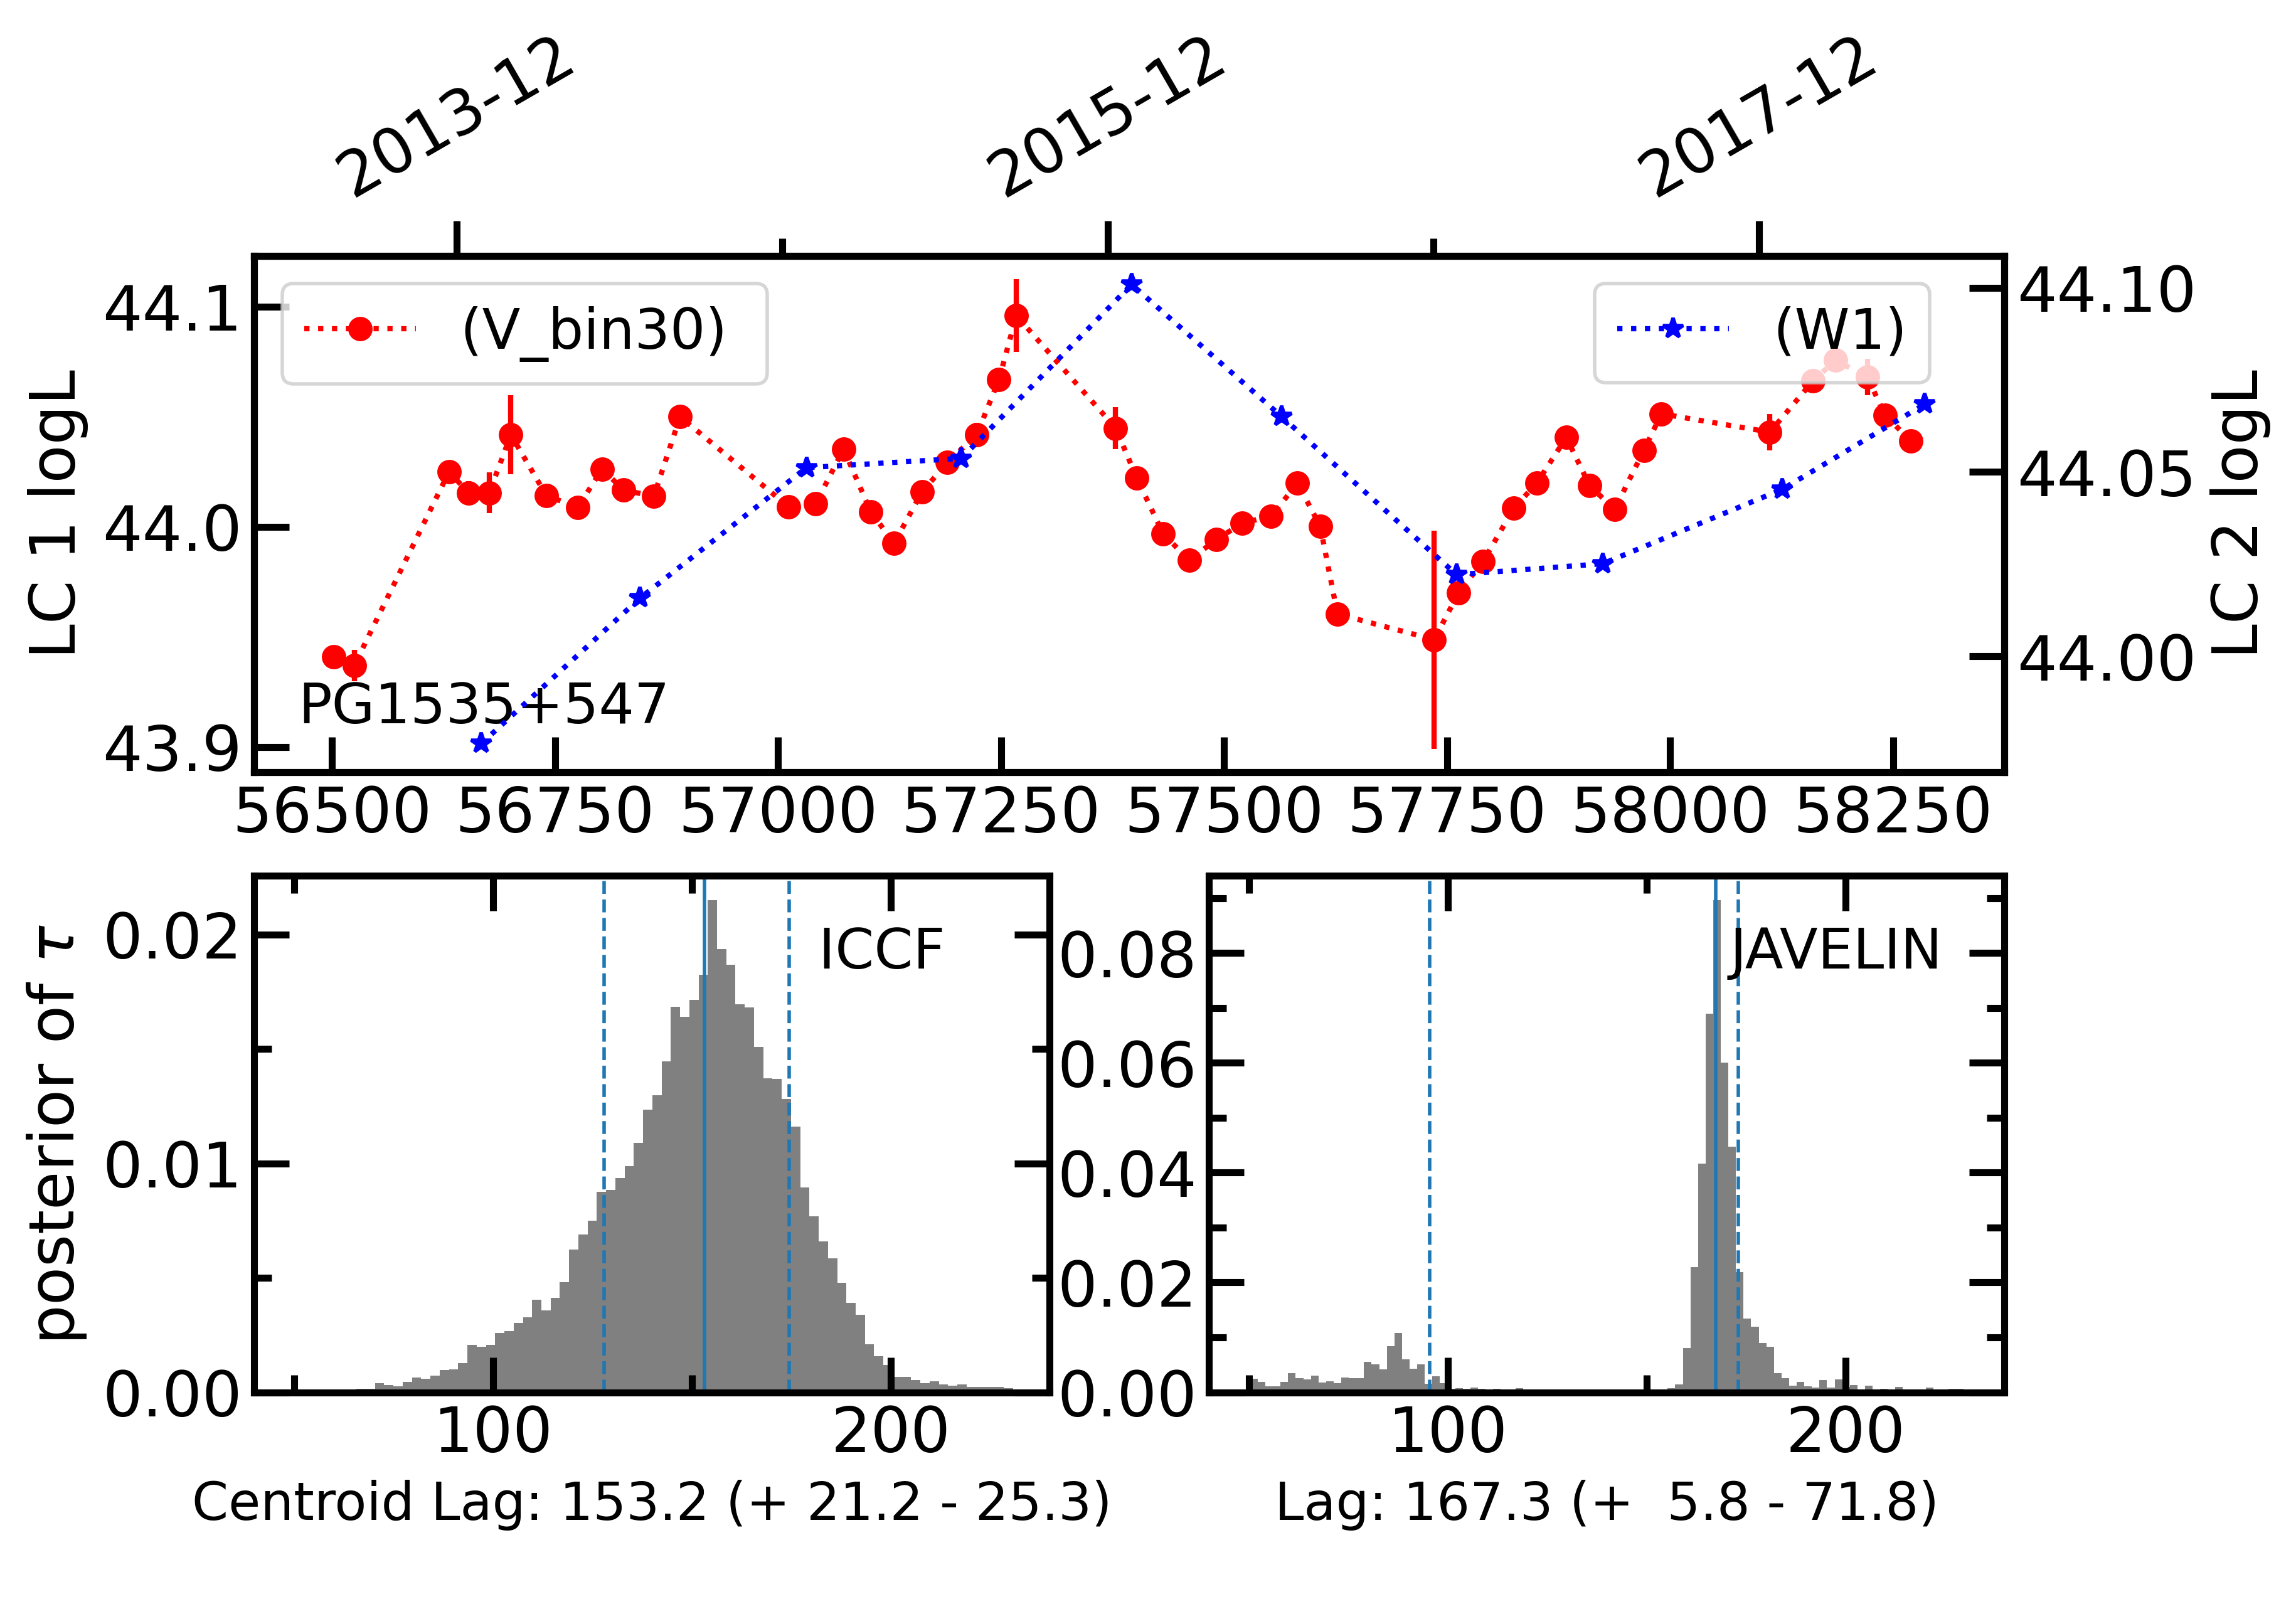
\includegraphics[width=0.5\textwidth]{pic/PG1535p547lag1.png}
    \caption{Dust-reverberation time lag analysis for PG 1535+547. }
    \label{fig:lag_PG1535}
\end{figure}